\documentclass[
12pt, % 字体大小
a4paper, 
oneside, % 单面打印(双面为twoside)
headinclude,footinclude, % 页眉页脚包含在文本区域内,确保不被裁剪或掩盖
]{scrartcl}
% 主题和样式
\usepackage[
nochapters, % 无章节层级 
beramono, % 等宽字体样式
eulermath, % 数学公式Euler字体
pdfspacing, % 字间距
dottedtoc % 点线式目录
]{classicthesis}
\usepackage{arsclassica} 
%----------------------------------------------------------------------------------------
% 输入和页面排版
\usepackage[T1]{fontenc} % 字体编码
\usepackage[utf8]{inputenc} % 输入编码
\usepackage{ctex} % 汉语
\usepackage{amsmath,amssymb,amsthm} % 数学公式
\usepackage{indentfirst} % 缩进
\setlength{\parindent}{2em} % 段落缩进
\usepackage[
top=2cm,
bottom=2cm, 
left=2cm,
right=2cm, 
headheight=20pt, 
includeheadfoot 
]{geometry} % 页面
\usepackage{scrlayer-scrpage} % 页眉页脚
\renewcommand{\sectionmark}[1]{\markright{\spacedlowsmallcaps{#1}}}
\renewcommand{\subsectionmark}[1]{\markright{\thesubsection~#1}}
\lehead{\mbox{\llap{\small\thepage\kern1em\color{halfgray} \vline}\color{halfgray}\hspace{0.5em}\rightmark\hfil}} % 标题旁边标记页码
\cfoot{\hyperlink{toc}{\color{RoyalBlue}返回目录}} % 页脚返回目录链接
\pagestyle{scrheadings}
%----------------------------------------------------------------------------------------
% 图表和引用
\usepackage{graphicx} % 图像
\graphicspath{{Figures/}} % 图像路径
\usepackage{subfig} % 图组
\usepackage{float} % 浮动
\usepackage{enumitem} % 列表
\usepackage{varioref} % 交叉引用
%----------------------------------------------------------------------------------------
% 代码
\usepackage{listings}
\lstset{
    language=Matlab,
    basicstyle=\ttfamily\small,   % 字体
    numbers=left,                 % 行号
    numberstyle=\tiny\color{gray},
    stepnumber=5,
    numbersep=5pt,
    backgroundcolor=\color{white},% 背景
    tabsize=2,                    % 制表符宽度
    frame=single,                 % 边框
    captionpos=t,                 % 标题
    title=\lstname,
    breaklines=true,              % 换行
    breakatwhitespace=true,
    escapeinside={`}{`},          % 转义(中文注释)
}
\lstset{
    language=Python,            
    basicstyle=\ttfamily\small,   % 字体
    numbers=left,                 % 行号
    numberstyle=\tiny\color{gray}, 
    stepnumber=5,             
    numbersep=5pt,            
    backgroundcolor=\color{white},% 背景
    tabsize=4,                    % 制表符宽度            
    frame=single,                 % 边框
    captionpos=t,                 % 标题
    title=\lstname, 
    breaklines=true,              % 换行
    breakatwhitespace=false,   
    escapeinside={`}{`},          % 转义(中文注释)
}
\usepackage{algorithm} % 算法
\usepackage{algpseudocode}
\usepackage{mdframed} % 跨页框架
% 不浮动算法环境
\newcounter{myalgorithm}
\renewcommand{\themyalgorithm}{\arabic{myalgorithm}}
\newenvironment{myalgorithm}[1][]{
  \refstepcounter{myalgorithm}
  \begin{mdframed}[
    skipabove=\topskip,
    skipbelow=\topskip,
    needspace=3\baselineskip,
    linewidth=0.4pt,
    frametitlefont=\normalfont\bfseries,
    frametitle={算法 \themyalgorithm\if\relax\detokenize{#1}\relax\else:#1\fi},
    frametitlerule=true,
    frametitlerulewidth=0.4pt,
    repeatframetitle=true
  ]
  \begin{algorithmic}[1]
  \ifx\relax\detokenize{#1}\relax
    \addcontentsline{alg}{algorithms}{\makebox[7em][l]{算法~\themyalgorithm} }
  \else
    \addcontentsline{alg}{algorithms}{\makebox[7em][l]{算法~\themyalgorithm} #1}
  \fi
}{
  \end{algorithmic}
  \end{mdframed}
}
% 关键词
\algrenewcommand{\algorithmicwhile}{当}
\algrenewcommand{\algorithmicdo}{执行}
\algrenewcommand{\algorithmicend}{结束}
\algrenewcommand{\algorithmicif}{如果}
\algrenewcommand{\algorithmicthen}{那么}
\algrenewcommand{\algorithmicelse}{否则}
\algrenewcommand{\algorithmicfor}{对于}
\algrenewcommand{\algorithmicrepeat}{循环}
\algrenewcommand{\algorithmicuntil}{直到}
\algrenewcommand{\algorithmicloop}{循环}
\algnotext{EndFor}
\algnotext{EndIf}
\algnotext{EndLoop}
\algnotext{EndWhile}
%----------------------------------------------------------------------------------------
% 超链接与PDF信息
\usepackage{hyperref} 
\hypersetup{
colorlinks=true, % 彩色
breaklinks=true, % 断行
urlcolor=webbrown, % URL棕色
linkcolor=RoyalBlue, % 内部链接蓝色
citecolor=webgreen, % 引用绿色
bookmarks=true, % 书签
bookmarksnumbered,
pdftitle={}, 
pdfauthor={},
pdfsubject={}, 
pdfkeywords={}, 
pdfcreator={pdfLaTeX}, 
pdfproducer={LaTeX with hyperref and ClassicThesis} 
}
%----------------------------------------------------------------------------------------
% 目录与标题
\usepackage{titlesec} 
\AtBeginDocument{
    \renewcommand{\contentsname}{目\hspace{1em}录}
    \renewcommand{\listfigurename}{图\hspace{1em}片}
    \renewcommand{\listtablename}{表\hspace{1em}格}
    \renewcommand{\figurename}{图}
    \renewcommand{\tablename}{表}
    \setcounter{tocdepth}{3} % 目录深度
}
\theoremstyle{definition} 
\newtheorem{definition}{定义}
\theoremstyle{plain} 
\newtheorem{theorem}{定理}
\theoremstyle{remark}
\newtheorem{remark}{备注}
\newtheorem{example}{样例}
\usepackage{tocloft} % 目录
% 要点目录
\newlistof{tips}{tip}{要\hspace{1em}点}
\newcommand{\tip}[1]{
  \refstepcounter{tips}
  \textsuperscript{\textcolor{orange}{\textbf{\thetips}}}
  \addcontentsline{tip}{tips}{\makebox[7em][l]{要点~\thetips} #1}
}
% 算法目录
\newlistof{algorithms}{alg}{算\hspace{1em}法} 
\hyphenation{Fortran hy-phen-ation} % 单词断字规则
%----------------------------------------------------------------------------------------
% 题目和作者
\title{\normalfont\spacedallcaps{智能工程}} 
\date{}
%----------------------------------------------------------------------------------------
% 开始和目录
\begin{document}
\maketitle
\newpage
\hypertarget{toc}{}
\begingroup
\begin{multicols}{2}
\tableofcontents
\end{multicols}
\endgroup
\hrule
\begingroup
\begin{multicols}{2}
\listoffigures
\end{multicols}
\endgroup
\hrule
\begingroup
\begin{multicols}{2}
\listoftables
\end{multicols}
\endgroup
\hrule
\begingroup
\begin{multicols}{2}
\listoftips
\end{multicols}
\endgroup
\newpage
%----------------------------------------------------------------------------------------
\section{基础知识}
%------------------------------------------------
\paragraph{课程内容}
\begin{figure}[H]
\centering
\subfloat[课程内容]{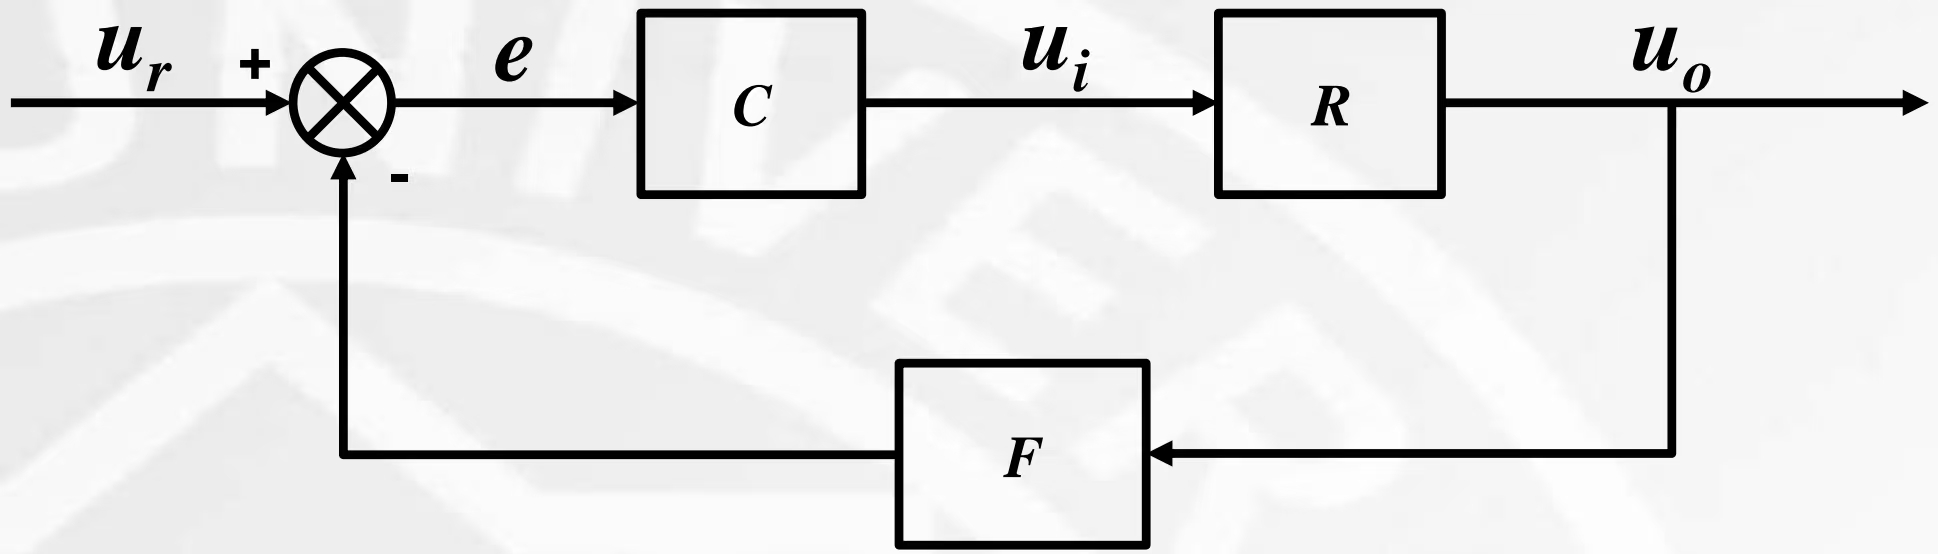
\includegraphics[width=.45\textwidth]{control}} \quad
\subfloat[工作流程]{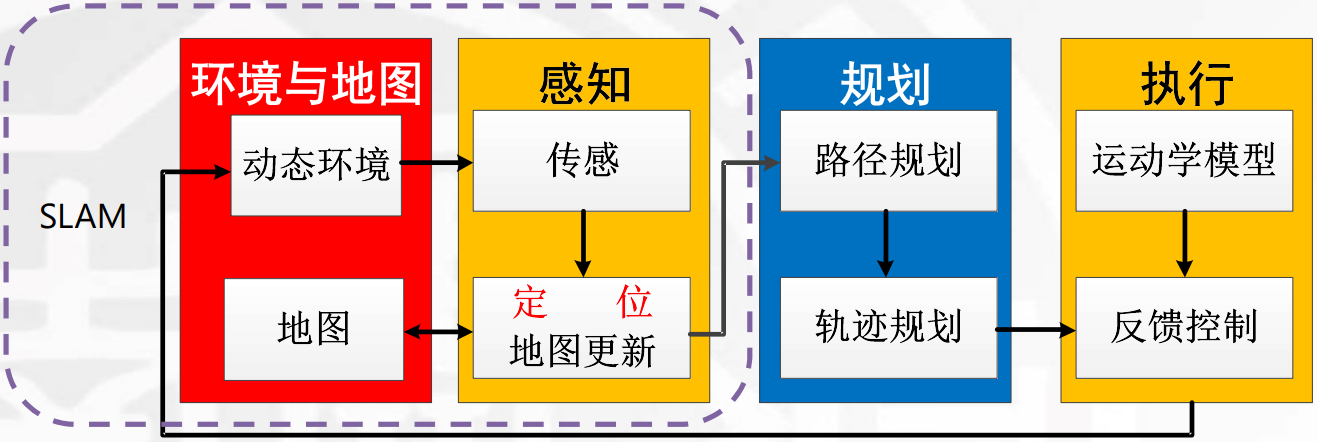
\includegraphics[width=.45\textwidth]{workflow}}
\caption{课程内容}
\end{figure}

\begin{table}[H]
\centering
\begin{tabular}{|p{0.5cm}|p{2cm}|p{2cm}|p{2cm}|p{2cm}|p{2cm}|p{2cm}|p{2cm}|}
\hline
& $ u_i $ & $ u_o $ & $ R $ & $ F $ & $ u_r $ & $ e $ & $ C $ \\
\hline
概念 & 系统输入 & 系统输出 & 系统模型 & 反馈单元 & 系统给定 & 系统误差 & 控制器 \\
\hline
含义 & 对被控对象施加作用的手段 & 作业目标的可测系统状态 & 系统输入输出映射 & 系统输出映射变换 & 系统作业目标 & 作业目标与系统当前测量状态差值 & 系统误差与输入映射 \\
\hline
内容 & \multicolumn{3}{c|}{机器人运动学} & \multicolumn{2}{c|}{机器人控制} & 机器人感知 & 机器人运动规划 \\
\hline
\end{tabular}
\caption{课程内容}
\end{table}
%------------------------------------------------
\paragraph{课程案例}\label{sec:two_wheel}
移动机器人->轮式机器人->两轮差速机器人。

\noindent
\begin{minipage}{0.3\textwidth}
\begin{figure}[H]
\centering
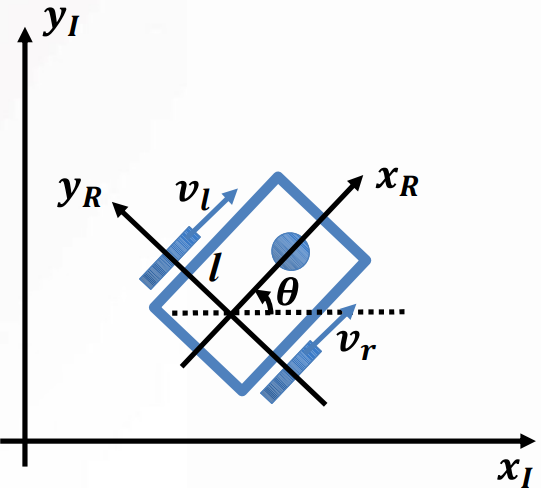
\includegraphics[width=0.6\linewidth]{two_wheel} 
\caption{两轮差速机器人模型}
\end{figure}
\end{minipage}
\begin{minipage}{0.4\textwidth}
\begin{itemize}
\item 车轮半径$ r $。
\item 两轮转速$ \varphi_l,\varphi_r $:$ v_i = r\varphi_i $。
\item 车轮到两轮中间点距离$ l $。
\end{itemize}
\end{minipage}
\begin{minipage}{0.3\textwidth}
\begin{enumerate}
\item 正运动学模型\ref{sec:example1}。
\item 运动控制器\ref{sec:motion_control}。
\item 里程计模型\ref{sec:odometer}。
\end{enumerate}
\end{minipage}
%------------------------------------------------
\begin{comment}
\section{机器人运动形态}
%------------------------------------------------
\subsection[移动机器人]{移动机器人}
%------------------------------------------------
\noindent
\begin{minipage}{0.4\textwidth}
\paragraph{自然界运动形态特点}
\begin{itemize}
\item 能量利用率高。
\item 适应野外复杂环境。
\item 与身体尺寸、结构相适应。
\item 运行速度高。
\end{itemize}
\end{minipage}
\begin{minipage}{0.6\textwidth}
\paragraph{机器人实现自然界运动形态问题}
\begin{itemize}
\item 机械结构、能量密度、感知与控制决策能力困难。
\item 安全性、可靠性差。
\item 成本高。
\item 于人造环境低效。
\end{itemize}
\end{minipage}
%------------------------------------------------
\paragraph{运动(Locomoion)}
机器人与环境的物理交互方式。
\begin{itemize}
\item 稳定性。
\item 接触特性。
\item 环境特性。
\end{itemize}
%------------------------------------------------
\subsection[腿式机器人]{腿式机器人}
%------------------------------------------------
\subsubsection[腿式机器人]{腿式机器人}
%------------------------------------------------
\paragraph{研究意义}
\begin{itemize}
\item 复杂恶劣环境的高适应性。
\item 点接触的高通过能力。
\item 控制多自由度、实时感知环境的高实现难度。
\end{itemize}
%------------------------------------------------
\paragraph{腿数影响}
\begin{itemize}
\item 机构复杂度。
\item 控制复杂度。
\item 环境适应性:腿越多,通过性越好,环境适应性越强。
\item 系统稳定性:腿数增加,由动态稳定向静态稳定过度。
\begin{itemize}
\item 动态稳定:执行器停止工作摔倒。运动过程中通常半数腿离地。
\item 静态稳定:执行器停止工作不摔倒。点接触需保证三腿同时着地,面接触需保证一条腿着地。
\end{itemize}
\end{itemize}
%------------------------------------------------
\paragraph{运动规划}
运动学+动力学。
%------------------------------------------------
\paragraph{步态}
一个行进周期内各腿抬落组合,$ k $腿机器人的步态模式数量为$ N = (2^k - 1)! $。
%------------------------------------------------
\paragraph{单位距离能耗}
$ COT = \frac{\text{消耗能量}}{\text{重量} \times \text{运行距离}} $。
%------------------------------------------------
\subsubsection[四足机器人]{四足机器人}
\begin{itemize}
\item 点接触:每条腿至少需要两个自由度,执行器较少,没有冗余。
\item 行走(静态平衡):一次移动一条腿,剩下腿支持身体,重心落在支持多边形内。适合攀爬,速度低,能效低。
\item 奔跑(动态平衡):一次移动多条腿,平衡建立在周期运动上。速度高,能效高,需要实时控制与执行。
\end{itemize}
%------------------------------------------------
\subsubsection[双足机器人]{双足机器人}
%------------------------------------------------
\paragraph{两种方案}
\begin{table}[H]
\centering
\begin{tabular}{|c|c|c|c|c|c|c|}
\hline
方案 & 国家 & 基础方式 & 重心 & 速度 & 环境适应性 & 能效 \\
\hline
静态稳定 & 日本 & 面接触 & 左右变换 & 低 & 差 & 低 \\
\hline
动态稳定 & 美国 & 点接触 & 适时调整 & 高 & 强 & 高 \\
\hline
\end{tabular}
\caption{双足机器人方案对比}
\end{table}
%------------------------------------------------
\paragraph{动态稳定运动机理}
\begin{itemize}
\item 倒立摆模型:类似纯滚动,步距越小越趋于圆。步态不自然,重心变化(需做功),落地冲击大。
\item 无源动态行走:摆动与向前摔落结合,势能转化为动能。
\item 弹簧负载倒立摆(SLIP):仿照动物腿肌肉,增加弹簧缓冲并储存能量。周期往复运动对称,动态稳定性可由庞加莱变换线性化后验证,条件为$ \lambda < 1 $(PPT.2.34-43)。
\item 串联弹性驱动(SEA):更为高效,更符合生物自然属性,基于运动学的位置控制,基于动力学的力矩控制。可由其获得稳定平台(PPT.2.48-50)。
\end{itemize}
%------------------------------------------------
\subsection[轮式机器人]{轮式机器人}
%------------------------------------------------
\paragraph{研究意义}
\begin{itemize}
\item 人造环境下高效:滚动摩擦,无重心起伏。
\item 结构简单,可靠性高,成本低。
\item 控制简单,系统复杂度低。
\end{itemize}
%------------------------------------------------
\paragraph{轮数对稳定性的影响}
轮数增加,由动态稳定向静态稳定过度。
\begin{itemize}
\item 动态稳定:执行器停止工作摔倒。倒立摆模型。    
\item 静态稳定:执行器停止工作不摔倒。陀螺效应,随动轮效应。
\end{itemize}
\end{comment}
%----------------------------------------------------------------------------------------
\section{机器人运动学}
%------------------------------------------------
\subsection[运动学模型]{运动学模型}
表征机器人驱动(输入)和机器人空间位姿(输出)的关系。
%------------------------------------------------
\paragraph{机械臂与移动机器人的区别}
\begin{itemize}
\item 机械臂本体坐标系固定,精度高;移动机器人本体坐标系随动,精度低。
\item 非完整约束\tip{非完整约束}:移动机器人只知道码盘变化量无法获取位姿,状态取决于路径,源于不可积的微分约束(车轮侧向滑动约束)。
\item 微分运动学(Differential Kinematics):速度空间替代位置空间。
\end{itemize}
%------------------------------------------------
\subsection[车轮]{车轮}
%------------------------------------------------
\paragraph{类型}\tip{车轮类型}
\begin{figure}[H]
\centering 
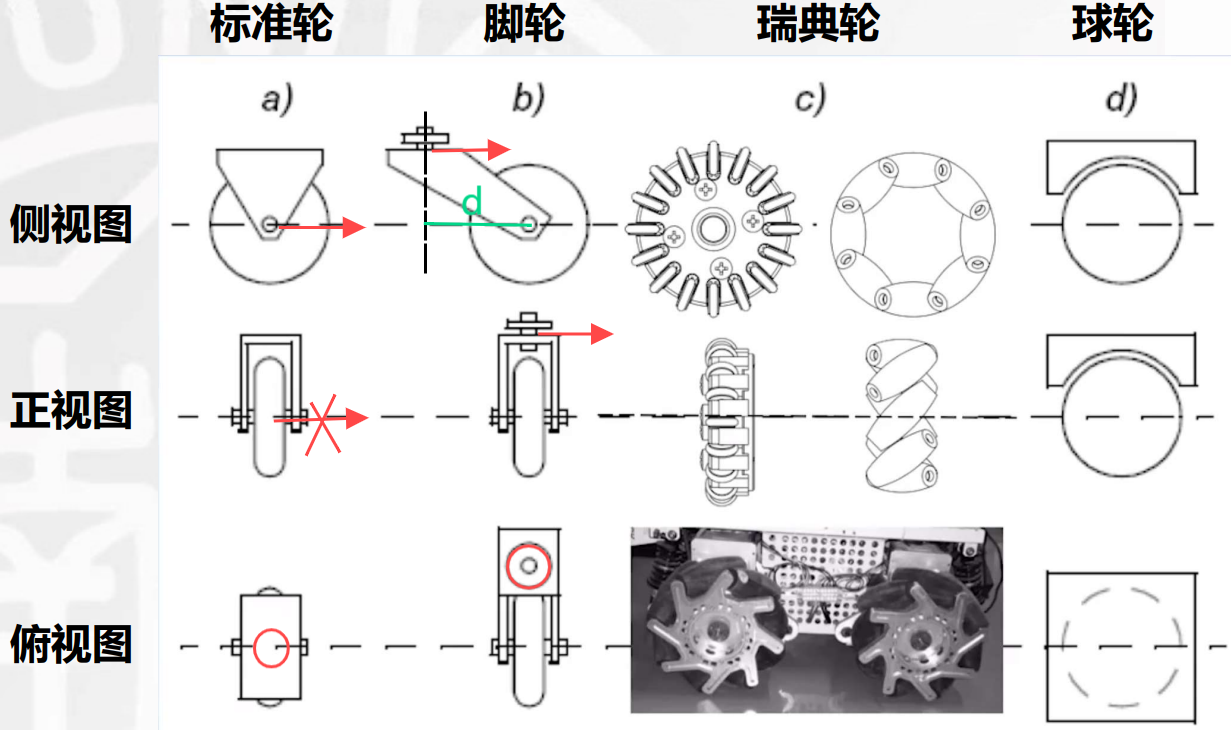
\includegraphics[width=0.6\textwidth]{tire} 
\caption{车轮类型}
\end{figure}

\begin{table}[H]
\centering
\begin{tabular}{|p{2cm}|p{4.2cm}|p{2.2cm}|p{7cm}|}
\hline
类型 & 自由度 & 约束 & 分类/特点 \\
\hline
标准轮 \newline (Standard wheel) & $ 2 $ \newline 沿轮平面滚动 \newline 沿垂直轴转动 & $ 1 $ \newline 沿轮轴滑动 & 标准固定轮(无法旋转,只有一个自由度) \newline 标准转向轮(舵轮) \\
\hline
脚轮 \newline (Castor wheel) & $ 3 $ \newline 沿轮平面滚动 \newline 沿垂直轴转动 \newline 沿路轴运动 & $ 0 $ & 偏心距 $ d $:触地点到垂直旋转轴距离。扭矩压力,易损坏。 \\
\hline
瑞典轮 \newline (Swedish wheel) & $ 3 $ \newline 沿轮平面滚动(被动) \newline 沿轮轴转动(主动) \newline 沿垂直轴转动(被动) & $ 0 $ & 麦克纳姆轮(Macanum wheel):$ 45° $,至少需要$ 4 $个共同使用。 \newline 连续切换轮:$ 90° $,至少需要$ 3 $个共同使用。 \newline 对地面冲击大,噪音大,易损坏,成本高。 \\
\hline
球轮 \newline (Spherical wheel) & $ 3 $(全主动) \newline 沿两个正交轮轴转动 \newline 沿垂直轴转动 & $ 0 $ & 成本高,可靠性差。 \\
\hline
\end{tabular}
\caption{车轮类型对比}
\end{table}
%------------------------------------------------
\paragraph{选取}
\begin{itemize}
\item 数量:至少三轮同时着地,才能保证静态稳定性。四轮可以提升稳定性,但需要悬架。
\item 大小:越大的轮子通过性越好,但需要更大的扭矩。
\item 多数形态都有非完整约束。
\end{itemize}
%------------------------------------------------
\subsection[运动学建模]{运动学建模}
%------------------------------------------------
\subsubsection[空间描述与状态表达]{空间描述与状态表达}
%------------------------------------------------
\paragraph{坐标系}
\begin{itemize}
\item 惯性系I:作业目标、控制指令、传感器感知测量信息。
\item 机器人系R:控制器误差输入、控制器控制指令。
\item 笛卡尔系:右手法则。
\end{itemize}
%------------------------------------------------
\paragraph{位姿(Pose)}~\\

位置空间求导得到速度空间:
$$
\xi_I = \begin{bmatrix} x_I \\ y_I \\ \theta_I \end{bmatrix}, 
\xi_R = \begin{bmatrix} x_R \\ y_R \\ \theta_R \end{bmatrix}
\overset{\text{求导}}{\Longrightarrow}
\xi_I = \begin{bmatrix} \dot{x}_I \\ \dot{y}_I \\ \dot{\theta}_I \end{bmatrix},
\xi_R = \begin{bmatrix} \dot{x}_R \\ \dot{y}_R \\ \dot{\theta}_R \end{bmatrix}
$$

惯性系旋转得到机器人系:
$$ \dot{\xi}_R = R(\theta) \dot{\xi}_I $$

旋转阵$ R(\theta) = \begin{bmatrix} \cos\theta & \sin\theta & 0 \\ -\sin\theta & \cos\theta & 0 \\ 0 & 0 & 1 \end{bmatrix} $为单位正交阵,$ R^T = R^{-1} $。
%------------------------------------------------
\subsubsection[瞬心法]{瞬心(ICR)法\tip{瞬心法运动学建模}}
\noindent
\begin{minipage}{0.4\textwidth}
\paragraph{瞬时旋转/曲率中心(ICR)}~\\
\hspace{2em}
刚体上各点角速度相同。
\begin{figure}[H]
\centering 
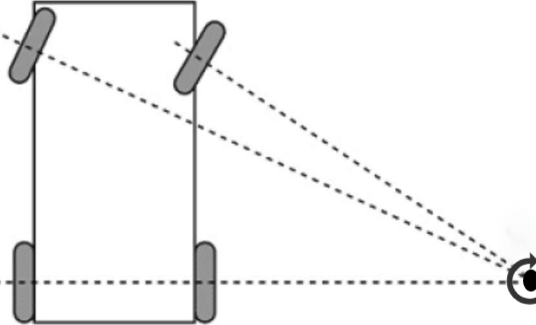
\includegraphics[width=0.5\textwidth]{icr_point} 
\caption{瞬心}
\end{figure}
\end{minipage}
\begin{minipage}{0.6\textwidth}
\paragraph{步骤}
\begin{enumerate}
\item 坐标系变换。
\item 确定约束。
\item 确定瞬心:各轮轮轴到该点距离与速度成正比。
\item 求解$ \dot{\xi}_R = \begin{bmatrix} \dot{x}_R & \dot{y}_R & \dot{\theta}_R \end{bmatrix}^T $。
\end{enumerate}
\end{minipage}
%------------------------------------------------
\subsubsection[约束方程法]{约束方程法\tip{约束方程法运动学建模}}
%------------------------------------------------
\paragraph{要求}
在水平面上运动,车轮与地面点接触,不变形,安装在钢体表面,舵机转轴与地面垂直。
%------------------------------------------------
\paragraph{约束方程}
\begin{figure}[H]
\centering
\subfloat[标准轮]{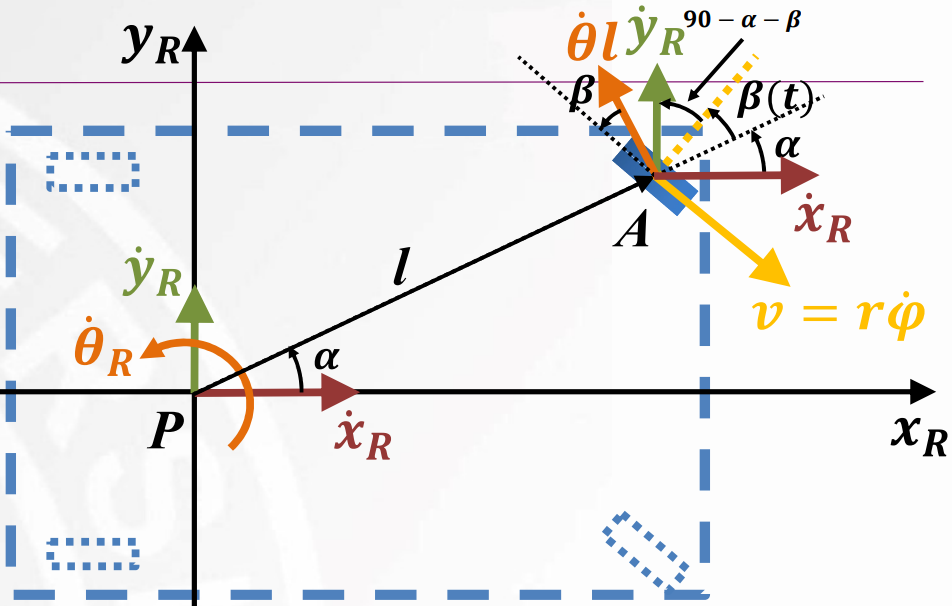
\includegraphics[width=.3\textwidth]{Standard_wheel}} \quad
\subfloat[脚轮]{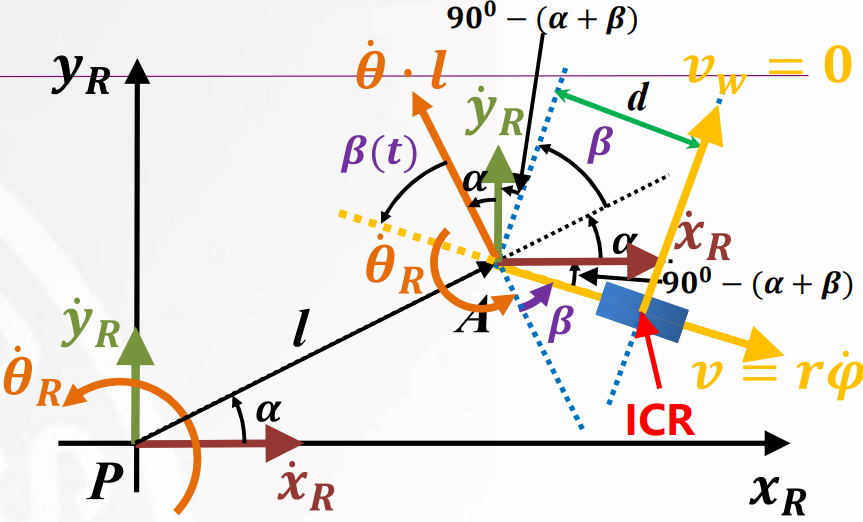
\includegraphics[width=.3\textwidth]{Castor_wheel}} \quad
\subfloat[瑞典轮]{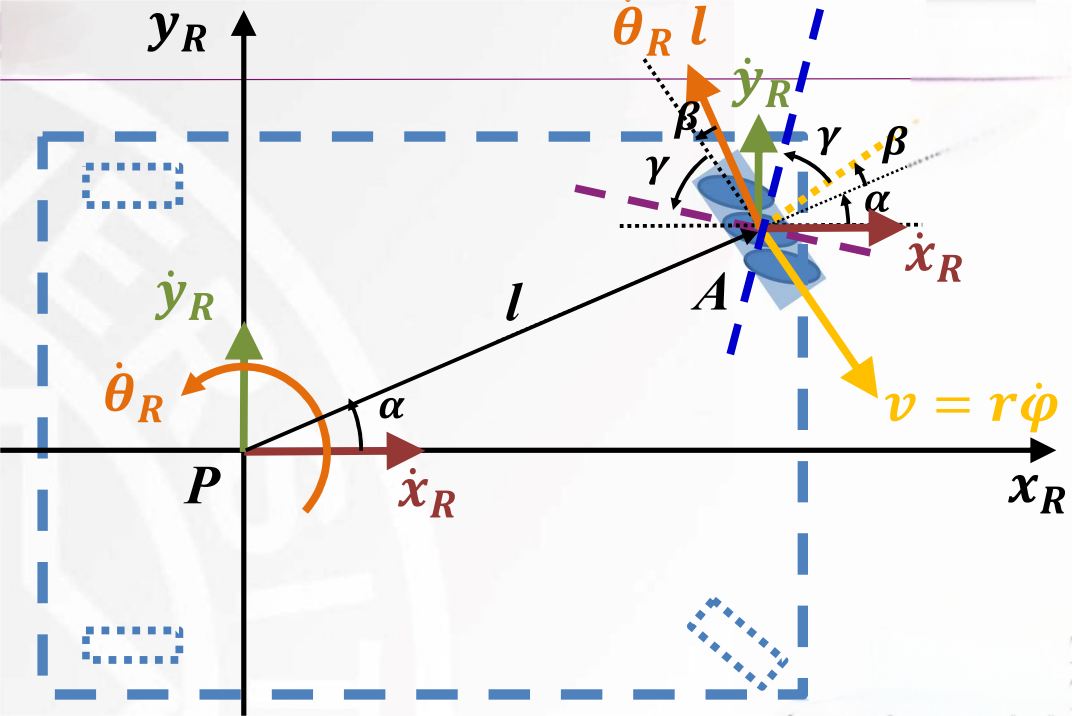
\includegraphics[width=.3\textwidth]{Swedish_wheel}}
\caption{车轮约束示意图}
\end{figure}

\begin{table}[H]
\centering
\begin{tabular}{|p{0.9cm}|p{1.3cm}|p{10cm}|p{1.4cm}|p{1.3cm}|}
\hline
类型 & 约束 & 约束方程 & 主动轮 & 随动轮 \\
\hline
\multirow{2}{*}{\parbox[c]{0.9cm}{标\\准\\轮}} & 纯滚动 & $ \begin{bmatrix} \sin(\alpha + \beta(t)) & -\cos(\alpha + \beta(t)) & -l\cos\beta(t) \end{bmatrix} R\theta \dot{\xi}_I \newline = r\dot{\varphi} $ & $ \surd $ & x \\
\cline{2-5}
& 无滑动 & $ \begin{bmatrix} \cos(\alpha + \beta(t)) & \sin(\alpha + \beta(t)) & l\sin\beta(t) \end{bmatrix} R\theta \dot{\xi}_I = 0 $ & $ \surd $ & $ \surd $ \\
\hline
\multirow{2}{*}{\parbox[c]{0.9cm}{脚\\轮}} & 纯滚动 & $ \begin{bmatrix} \sin(\alpha + \beta) & -\cos(\alpha + \beta) & -l\cos\beta \end{bmatrix} R\theta \dot{\xi}_I = r\dot{\varphi} $ & $ \surd $ & x \\
\cline{2-5}
& 无滑动 & $ \begin{bmatrix} \cos(\alpha + \beta) & \sin(\alpha + \beta) & d + l\sin\beta \end{bmatrix} R\theta \dot{\xi}_I = -d\dot{\beta} $ & $ \surd $ & x \\
\hline
\multirow{2}{*}{\parbox[c]{0.9cm}{瑞\\典\\轮}} & 纯滚动 & $ \begin{bmatrix} \cos(\alpha + \beta + \gamma) & \sin(\alpha + \beta + \gamma) & l\sin(\beta + \gamma) \end{bmatrix} R\theta \dot{\xi}_I \newline = r\dot{\varphi}\sin\gamma + r_{sw}\dot{\varphi}_{sw} $ & $ \surd $ & x \\
\cline{2-5}
& 无滑动 & $ \begin{bmatrix} \sin(\alpha + \beta + \gamma) & -\cos(\alpha + \beta + \gamma) & -l\cos(\beta + \gamma) \end{bmatrix} R\theta \dot{\xi}_I \newline = r\dot{\varphi}\cos\gamma $ & $ \surd $ \newline 小轮 & x \\
\hline
\end{tabular}
\caption{车轮约束方程}
\end{table}
%------------------------------------------------
\paragraph{使用}
根据各轮主/随动状态列运动约束方程,得到最多三个独立约束方程(对应平面三维位姿)。

以下以$ N $个标准轮($ N_f $个固定,$ N_s $个转向)机器人为例:
\begin{itemize}
\item 滚动约束
$$ J_1(\beta_s) R(\theta) \dot{\xi}_I - J_2 \dot{\varphi} = 0 $$

其中$ J_1(\beta_s) =  \begin{bmatrix} {J_{1f}}_{(N_f \times 3)} \\ {J_{1s}(\beta_s)}_{(N_s \times 3)} \end{bmatrix}, \varphi(t) = \begin{bmatrix} \varphi_f(t) \\ \varphi_s(t) \end{bmatrix}, J_2 = diag(r_1, \cdots, r_N)\text{为轮径对角阵} $。
\item 滑动约束
$$ C_1(\beta_s) R(\theta) \dot{\xi}_I = 0 $$

其中$ C_1(\beta_s) = \begin{bmatrix} {C_{1f}}_{(N_f \times 3)} \\ {C_{1s}(\beta_s)}_{(N_s \times 3)} \end{bmatrix} $。
\end{itemize}
%------------------------------------------------
\subsubsection[例子]{例子}\label{sec:example1}
以下以两轮差速机器人(见\ref{sec:two_wheel})为例,$ \alpha = \frac{\pi}{2}, \beta = 0 $:
\begin{figure}[H]
\centering
\subfloat[瞬心法]{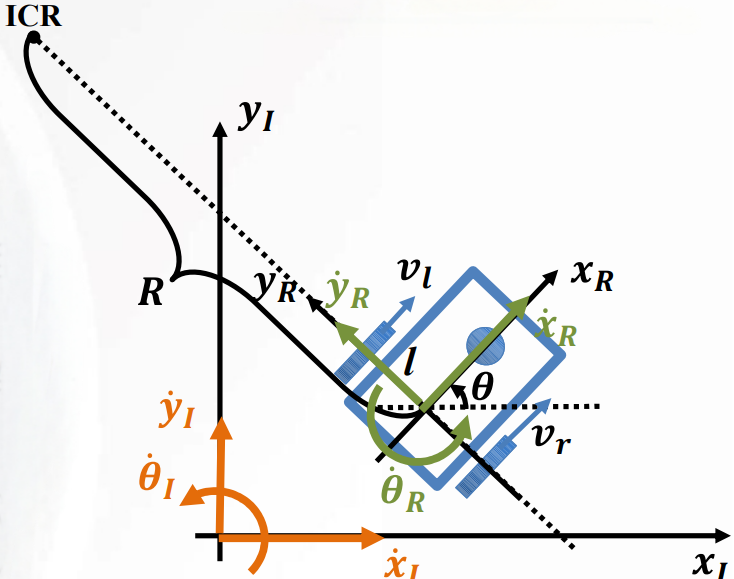
\includegraphics[width=.3\textwidth]{icr}} \quad
\subfloat[约束方程法]{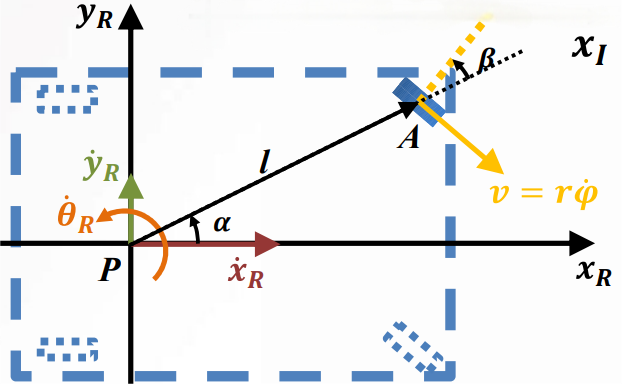
\includegraphics[width=.35\textwidth]{Equation_of_motion}}
\caption{两轮差速机器人正运动学建模}
\end{figure}
%------------------------------------------------
\paragraph{瞬心法}~\\

两轮差速机器人的瞬心在两轮轮轴上,设其到机器人两轮中间的距离为$ R $,有:
$$ \dot{\theta} = \frac{\dot{x}_R}{R} = \frac{\dot{\varphi}_l r}{R-l} = \frac{\dot{\varphi}_r r}{R+l} $$

解得$ R = \frac{\dot{\varphi}_r + \dot{\varphi}_l}{\dot{\varphi}_r - \dot{\varphi}_l} $,代回即可。
%------------------------------------------------
\paragraph{约束方程法}
\begin{itemize}
\item 纯滚动:$ \begin{bmatrix} \sin(\alpha + \beta) & -\cos(\alpha + \beta) & -l\cos\beta \end{bmatrix} \dot{\xi}_R = r\dot{\varphi} $。
\item 无滑动:$ \begin{bmatrix} \cos(\alpha + \beta) & \sin(\alpha + \beta) & l\sin\beta \end{bmatrix} \dot{\xi}_R = 0 $。
\end{itemize}
%------------------------------------------------
\paragraph{正运动学模型}
$$ \dot{\xi}_R = \begin{bmatrix} \dot{x}_R \\ \dot{y}_R \\ \dot{\theta}_R \end{bmatrix} = \frac{r}{2} \begin{bmatrix} \dot{\varphi}_l + \dot{\varphi}_r \\ 0 \\ \frac{\dot{\varphi}_r - \dot{\varphi}_l}{l} \end{bmatrix} $$
%------------------------------------------------
\subsection[自由度]{自由度}
%------------------------------------------------
\paragraph{概念}
\begin{itemize}
\item 衡量机器人改变运行状态的能力。
\item 需满足实际作业需求,考虑实现成本。
\item 机器人设计基础、算法依据(一般同自由度机器人可采用相同控制规划算法)。
\item 平面运动机器人自由度最大不能超过$ 3 $。
\end{itemize}
%------------------------------------------------
\paragraph{分类}\tip{自由度}
\begin{itemize}
\item 移动度(Degree of Mobility)$ \delta_m $:瞬时改变机器人运动状态的能力。
$$ \delta_m = \dim[C_1(\beta_s)] = 3 - \operatorname{rank}[C_1(\beta_s)] \in [0,3] $$
\item 转向度(Degree of Steerability)$ \delta_s $:间接改变机器人运动状态的能力。
$$ \delta_s = \operatorname{rank}[C_{1s}(\beta_s)] \in [0,2] $$
\item 机动度(Degree of Maneuverability)$ \delta_M $:改变机器人运动状态的能力。
$$ \delta_M = \delta_m + \delta_s $$
\begin{itemize}
\item 机动度相同,结构不一定相同。
\item $ \delta_M = 2 $,瞬心位于一条直线上;$ \delta_M = 3 $,瞬心可分布于空间任何一点。
\end{itemize}
\end{itemize}
%------------------------------------------------
\paragraph{实例(Type(移动度,转向度))}
\begin{itemize}
\item 全向机器人:
\begin{itemize}
\item Type(3,0):完整约束全方位移动机器人。
\item Type(2,1):一个同心轮+两个瑞典轮。
\item Type(1,2):多舵机全方位移动机器人。
\end{itemize}
\item 非全向机器人:
\begin{itemize}
\item Type(2,0):差分移动机器人。
\item Type(1,1):自动驾驶汽车(阿克曼转向)、自行车、叉车。
\end{itemize}
\end{itemize}
%----------------------------------------------------------------------------------------
\section{机器人运动控制}
%------------------------------------------------
\subsection[运动控制]{运动控制}\label{sec:motion_control}
\begin{figure}[H]
\centering 
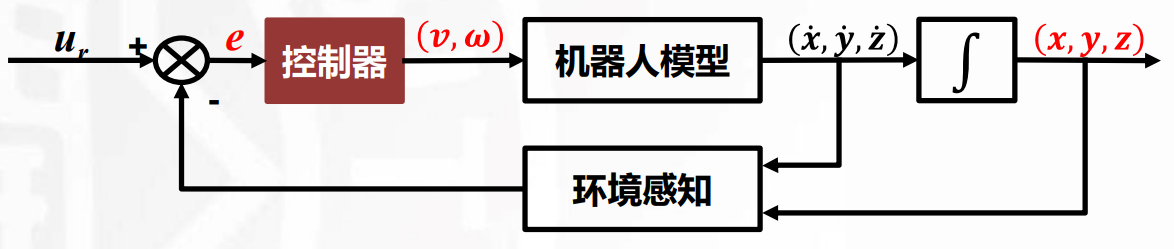
\includegraphics[width=0.6\textwidth]{controller} 
\caption{运动控制器}
\end{figure}

误差(惯性系下给定与反馈)$ \overset{\text{变换}}{\Longrightarrow} $输入(机器人系下控制输入)。 
%------------------------------------------------
\paragraph{特点}
\begin{itemize}
\item 大多存在滑动约束,是非完整系统,有侧向和姿态偏差。
\item 非线性,控制器设计复杂,还需要根据可获得的反馈信号选取,按顺序调节控制参数,并且不能同时实现定点控制和跟踪控制。
\item 不存在能完成控制目标的连续时不变(静态)反馈控制率。
\item 受标定精度影响大,且由于执行单元性能约束,控制输入要合理限幅。
\end{itemize}
%------------------------------------------------
\paragraph{分类}
\begin{itemize}
\item 定点(镇定)控制(Regulation Control):以指定姿态到达指定位置。
\item 跟踪控制:
\begin{itemize}
\item 轨迹跟踪控制(Trajectory Tracking Control):跟随给定轨迹(速度+姿态)。
\item 路径跟踪控制(Path Tracking Control):跟随给定路线。
\end{itemize}
\end{itemize}
%------------------------------------------------
\paragraph{开环控制}
将运动轨迹分割成直线和圆弧,存在以下问题:
\begin{itemize}
\item 直线和圆弧的曲率不一致,不连续。
\item 难以实现定义若干合适轨迹。
\item 速度加速度约束。
\item 无法自适应调整轨迹来面对环境变化。
\item 所得轨迹不光滑。
\end{itemize}
%------------------------------------------------
\paragraph{控制器性能评价}
取正定李雅普诺夫函数,其导数负定则系统渐进稳定。
%------------------------------------------------
\paragraph{两轮差速机器人运动控制}
以下以两轮差速机器人(见\ref{sec:two_wheel})为例。
$$ 
\dot{\xi}_R = \begin{bmatrix} \dot{x}_R \\ \dot{y}_R \\ \dot{\theta}_R \end{bmatrix} = \frac{r}{2} \begin{bmatrix} \dot{\varphi}_l + \dot{\varphi}_r \\ 0 \\ \frac{\dot{\varphi}_r-\dot{\varphi}_l}{l} \end{bmatrix} = \begin{bmatrix} v_1 \\ 0 \\ v_2 \end{bmatrix} 
\overset{\text{变换}}{\Longrightarrow}
\dot{\xi}_I = \begin{bmatrix} \dot{x}_I \\ \dot{y}_I \\ \dot{\theta}_I \end{bmatrix} = \begin{bmatrix} \cos\theta & 0 \\ \sin\theta & 0 \\ 0 & 1 \end{bmatrix} \begin{bmatrix} v_1 \\ v_2 \end{bmatrix} 
$$
%------------------------------------------------
\subsection[定点控制器]{定点控制器\tip{定点控制器(误差信号转换)}}
%------------------------------------------------
\paragraph{控制目标}
机器人参考坐标系下误差$ e = \begin{bmatrix} x & y & \theta \end{bmatrix}^T $,设计控制阵$ K = \begin{bmatrix} k_{11} & k_{12} & k_{13} \\ k_{21} & k_{22} & k_{23} \end{bmatrix} $,其中$ k_{ij} = k(t, e) $,得到控制输入$ \begin{bmatrix} v(t) \\ \omega(t) \end{bmatrix} = Ke $,使$ \lim_{t \to \infty} e(t) = 0 $。
%------------------------------------------------
\paragraph{误差信号转换}~\\

惯性系下,实际状态$ q = \begin{bmatrix} x & y & \theta \end{bmatrix}^T $与参考状态$ q_r \begin{bmatrix} x_r & y_r & \theta_r \end{bmatrix}^T $之差为开环误差$ \tilde{q} = \begin{bmatrix} \tilde{x} & \tilde{y} & \tilde{\theta} \end{bmatrix}^T = \begin{bmatrix} x - x_r & y - y_r & \theta - \theta_r \end{bmatrix}^T $。
\begin{enumerate}
\item 转换到机器人系
$$ 
e = \begin{bmatrix} e_1 \\ e_2 \\ e_3 \end{bmatrix} = R(\theta)^T \tilde{q} = \begin{bmatrix} \cos\theta & \sin\theta & 0 \\ -\sin\theta & \cos\theta & 0 \\ 0 & 0 & 1 \end{bmatrix} \begin{bmatrix} \tilde{x} \\ \tilde{y} \\ \tilde{\theta} \end{bmatrix}
\overset{\text{闭环}}{\Longrightarrow}
\dot{e} = \begin{bmatrix} \dot{e}_1 \\ \dot{e}_2 \\ \dot{e}_3 \end{bmatrix} = R(\theta)\dot{\tilde{q}} + \dot{R(\theta)}\tilde{q} = \begin{bmatrix} v_1 + v_2 e_2 \\ -v_2 e_1 \\ v_2 \end{bmatrix} 
$$
\item 转换到极坐标系
$$ 
\begin{cases}
\rho &= \sqrt{\tilde{x}^2 + \tilde{y}^2} \\
\beta &= -\arctan2(-\tilde{y},-\tilde{x}) \\
\alpha &= -\beta - \tilde{\theta} \\
\end{cases}
\overset{\text{闭环}}{\Longrightarrow}
\begin{bmatrix} \dot{\rho} \\ \dot{\beta} \\ \dot{\alpha} \end{bmatrix} = 
\begin{bmatrix} -\cos\alpha & 0 \\ \frac{\sin\alpha}{\rho} & 0 \\ \frac{\sin\alpha}{\rho} & -1 \end{bmatrix}
\begin{bmatrix} v_1 \\ v_2 \end{bmatrix}
$$ 
\end{enumerate}
%------------------------------------------------
\paragraph{机器人系非线性控制器}~\\

设计控制器$ \begin{bmatrix} v_1 \\ v_2 \end{bmatrix} = \begin{bmatrix} -k_1 e_1 \\ -k_2 e_2 + e_2^2 \sin(t) \end{bmatrix} $,代入得$ \begin{bmatrix} \dot{e}_1 \\ \dot{e}_2 \\ \dot{e}_3 \end{bmatrix} = \begin{bmatrix} -k_1 e_1 + v_2 e_2 \\ -v_2 e_1 \\ -k_2 e_2 + e_2^2 \sin(t) \end{bmatrix} $,其有误差时扰动,效果不佳。
%------------------------------------------------
\paragraph{极坐标系线性控制器}~\\

设计控制器%
$ 
\begin{cases}
v_1 &= k_\rho \rho \\
v_2 &= k_\alpha \alpha + k_\beta \beta
\end{cases}
$,%
代入得
$$ 
\begin{bmatrix} \dot{\rho} \\ \dot{\beta} \\ \dot{\alpha} \end{bmatrix} 
= \begin{bmatrix} -k_\rho \rho \cos\alpha \\ -k_\rho \sin\alpha \\ k_\rho \sin\alpha - k_\alpha \alpha - k_\beta \beta \end{bmatrix} 
\overset{\alpha \to 0}{\Longrightarrow}
\begin{bmatrix} -k_\rho \rho \\ -k_\rho \alpha \\ k_\rho \alpha - k_\alpha \alpha - k_\beta \beta \end{bmatrix} 
$$

其中前两行非线性耦合,在$ \alpha \to 0 $时指数性稳定,非全局稳定。
%------------------------------------------------
\paragraph{极坐标系线性控制器}~\\

设计控制器%
$
\begin{cases}
v_1 &= k_\rho \rho \cos\alpha \\
v_2 &= k_\alpha \alpha + \frac{k_\rho \sin \alpha \cos\alpha}{\alpha}(\alpha - k_\beta\beta)
\end{cases}
$,%
代入得
$$ 
\begin{bmatrix} \dot{\rho} \\ \dot{\beta} \\ \dot{\alpha} \end{bmatrix} 
= \begin{bmatrix} -k_\rho \rho \cos^2\alpha \\ -k_\rho \cos\alpha \sin\alpha \\ k_\rho \cos\alpha \sin\alpha - k_\alpha \alpha - \frac{k_\rho \sin\alpha \cos\alpha}{\alpha} (\alpha - k_\beta\beta) \end{bmatrix} 
\overset{\alpha \to 0}{\Longrightarrow}
\begin{bmatrix} -k_\rho \rho \\ -k_\rho \alpha \\ - k_\alpha \alpha + k_\rho k_\beta\beta \end{bmatrix} 
$$

其全局渐近稳定。
%------------------------------------------------
\subsection[轨迹跟踪控制器]{轨迹跟踪控制器\tip{轨迹跟踪控制器}}
%------------------------------------------------
\paragraph{控制目标与误差变换}~\\

惯性系下,实际轨迹$ q(t) = \begin{bmatrix} x(t) & y(t) & \theta(t) \end{bmatrix}^T $与参考轨迹$ q_r \begin{bmatrix} x_r(t) & y_r(t) & \theta_r(t) \end{bmatrix}^T $之差为开环误差$ \tilde{q}(t) = \begin{bmatrix} \tilde{x}(t) & \tilde{y}(t) & \tilde{\theta}(t) \end{bmatrix}^T = \begin{bmatrix} x(t) - x_r(t) & y(t) - y_r(t) & \theta(t) - \theta_r(t) \end{bmatrix}^T $,控制目标为$ \lim_{n \to \infty} \tilde{q}(t) = 0 $。

辅助误差信号为:
$$ 
e = \begin{bmatrix} \cos\theta & \sin\theta & 0 \\ -\sin\theta & \cos\theta & 0 \\ 0 & 0 & 1 \end{bmatrix} \begin{bmatrix} \tilde{x} \\ \tilde{y} \\ \tilde{\theta} \end{bmatrix}
\overset{\text{闭环}}{\Longrightarrow}
\dot{e} = \begin{bmatrix} v_1 + v_2 e_2 - v_{1r} \cos e_3 \\ - v_2 e_1 + v_{1r} \sin e_3 \\ v_2 - v_{2r} \end{bmatrix} 
$$
%------------------------------------------------
\paragraph{控制器}~\\

设计控制器$ \begin{bmatrix} v_1 \\ v_2 \end{bmatrix} = \begin{bmatrix} -k_1 e_1 + v_{1r} \cos e_3 \\ -v_{1r} \frac{\sin e_3}{e_3} e_2 - k_2 e_3 + v_{2r} \end{bmatrix} $,代入得$ \begin{bmatrix} \dot{e}_1 \\ \dot{e}_2 \\ \dot{e}_3 \end{bmatrix} = \begin{bmatrix} -k_1 e_1 + v_2 e_2 \\ -v_2 e_1 + v_{1r} \sin e_3 \\ -k_2 e_3 - v_{1r} \frac{\sin e_3}{e_3} e_2 \end{bmatrix} $。

$ e_3 \to 0 $时,控制器简化为$ \begin{bmatrix} v_1 \\ v_2 \end{bmatrix} = \begin{bmatrix} -k_1 e_1 + v_{r1} \\ -v_{r1}  e_2 + v_{r2} \end{bmatrix} $,代入得$ \begin{bmatrix} \dot{e}_1 \\ \dot{e}_2 \\ \dot{e}_3 \end{bmatrix} = \begin{bmatrix} -k_1 e_1 + v_2 e_2 \\ -v_2 e_1 \\ -k_2 e_3 - v_{r1} e_2 \end{bmatrix} $。
%------------------------------------------------
\subsection[路径跟踪控制器]{路径跟踪控制器\tip{路径跟踪控制器}}
%------------------------------------------------
\paragraph{控制目标与误差变换}~\\

惯性系下,实际路径$ q(s) = \begin{bmatrix} x(s) & y(s) & \theta(s) \end{bmatrix}^T $与参考路径$ q_r \begin{bmatrix} x_r(s) & y_r(s) & \theta_r(s) \end{bmatrix}^T $之差为开环误差$ \tilde{q}(s) = \begin{bmatrix} \tilde{x}(s) & \tilde{y}(s) & \tilde{\theta}(s) \end{bmatrix}^T = \begin{bmatrix} x(s) - x_r(s) & y(s) - y_r(s) & \theta(s) - \theta_r(s) \end{bmatrix}^T $,其中$ s \in [0,1] $为路径参考变量,控制目标为$ \lim_{n \to \infty} \tilde{q}(s) = 0 $。

作变换%
$
\begin{cases}
y_1 &= x + b\cos\theta \\
y_2 &= y + b\sin\theta
\end{cases}
$,%
进而得到闭环误差$ \begin{bmatrix} \dot{y}_1 \\ \dot{y}_2 \end{bmatrix} = \begin{bmatrix} \cos\theta & -b\sin\theta \\ \sin\theta & b\cos\theta \end{bmatrix} \begin{bmatrix} v \\ \omega \end{bmatrix} = T(\theta) \begin{bmatrix} v \\ \omega \end{bmatrix} $。

逆运算得到$ \begin{bmatrix} v \\ \omega \end{bmatrix} = T^{-1}(\theta) \begin{bmatrix} u_1 \\ u_2 \end{bmatrix} = \begin{bmatrix} \cos\theta & \sin\theta \\ -\frac{\sin\theta}{b} & \frac{\cos\theta}{b} \end{bmatrix} \begin{bmatrix} u_1 \\ u_2 \end{bmatrix} $,故%
$
\begin{cases}
\dot{y}_1 &= u_1 \\
\dot{y}_2 &= u_2 \\
\dot{\theta} &= \frac{u_2 \cos\theta - u_1 \sin\theta}{b}
\end{cases}
$。
%------------------------------------------------
\paragraph{控制器}~\\

设计控制器
$ 
\begin{cases}
u_1 = \dot{y}_{1d} + k_1(y_{1d} - y_1) \\
u_2 = \dot{y}_{2d} + k_2(y_{2d} - y_2)
\end{cases} 
$%
,有%
$
\begin{cases}
\dot{\tilde{y}}_1 = -k_1\tilde{y}_1 \\
\dot{\tilde{y}}_2 = -k_2\tilde{y}_2
\end{cases}
$%
,系统指数性收敛。
%----------------------------------------------------------------------------------------
\section{机器人感知}
%------------------------------------------------
\subsection[传感器]{传感器\tip{传感器}}
%------------------------------------------------
\paragraph{分类}
\begin{table}[H]
\begin{tabular}{|p{1.5cm}|p{4.2cm}|p{0.9cm}|p{0.8cm}|}
\hline
分类 & 传感器 & 感受 & 源 \\
\hline
\multirow{3}{*}{触觉} & 接触开关,碰撞器 & EC & P \\
 & 光学屏障 & EC & A \\
 & 非接触式接近传感器 & EC & A \\
\hline
\multirow{7}{*}{轮/电机} & 电刷编码器 & PC & P \\
 & 电位计 & PC & P \\
 & 同步器,旋转变压器 & PC & P \\
 & 光电编码器 & PC & P \\
 & 磁编码器 & PC & P \\
 & 电感编码器 & PC & P \\
 & 电容编码器 & PC & P \\
\hline
\multirow{3}{*}{方向} & 罗盘(Compass) & EC & P \\
 & 陀螺仪(Gyroscope) & PC & P \\
 & 倾角仪 & EC & A/P \\
\hline
\multirow{3}{*}{视觉} & 相机(Camera) & EC & P \\
 & 视觉测距套件 & EC & P \\
 & 目标跟踪套件 & EC & P \\
\hline
\end{tabular}
\begin{tabular}{|p{1.5cm}|p{4.2cm}|p{0.9cm}|p{0.8cm}|}
\hline
分类 & 传感器 & 感受 & 源 \\
\hline
\multirow{5}{*}{测距} & 反射率传感器 & EC & A \\
 & 超声波传感器 & EC & A \\
 & 激光测距仪 & EC & A \\
 & 光学三角测量 & EC & A \\
 & 结构光 & EC & A \\
\hline
\multirow{6}{*}{运动} & 多普勒雷达(Rader) & EC & A \\
 & 多普勒声波 & EC & A \\
 & 激光雷达(Laser) & EC & A \\
 & 里程计(Odometer) & PC & P \\
 & 惯导系统(IMU) & PC & P \\
 & 加速度传感器 & PC & P \\
\hline
\multirow{5}{*}{信标} & GPS & EC & A \\
 & 有源光学或射频信标 & EC & A \\
 & 有源超声波信标 & EC & A \\
 & 有源光学或射频信标 & EC & A \\
 & 反射信标 & EC & A \\
\hline
\end{tabular}
\caption{传感器分类}
\end{table}

\begin{itemize}
\item PC(Proprioceptive,本体感受)/EC(Exteroceptive,外感受)。
\item A(Active,有源)/P(Passive,无源)。
\end{itemize}
%------------------------------------------------
\paragraph{特性}
\begin{itemize}
\item 测量范围:测量上下界之差。    
\item 动态范围:测量范围上下界比率,常用对数表示,单位为$ dB $。
\item 分辨率:最小可测量变化量,一般为为动态范围下界。
\item 线性度:输入输出信号的映射关系。
\end{itemize}
%------------------------------------------------
\subsection[光电传感器]{光电传感器}
%------------------------------------------------
\subsubsection[概述]{概述}
把被测量变化转换成光信号变化,再转换成电信号。
%------------------------------------------------
\paragraph{组成}
辐射源、光学通路、光电器件。
%------------------------------------------------
\paragraph{特性}
\begin{itemize}
\item 不受电磁干扰影响。
\item 非接触测量。
\item 频谱宽,高精度,高分辨率,高可靠性,发应快。
\end{itemize}
%------------------------------------------------
\subsubsection[编码器]{编码器\tip{编码器}}
测量系统相对运动角度,具有高精度、高分辨率和高可靠性。按结构可分为接触式、光电式和电磁式,后两种为非接触式编码。
%------------------------------------------------
\paragraph{增量式旋转编码器}
\begin{itemize}
\item 不能直接输出数字编码,需要数字电路。
\item 原理:遮光周期性变化,莫尔条纹明暗交替,电压周期性变化$ U_0 = U_m \cos(\frac{2\pi}{W}x) $,形成脉冲,根据脉冲数量可推算旋转角度,位置数据是相对的,掉电后需要复位。
\item 辨向:为判断光栅移动方向,使用D触发器整合两个光栅的信息。
\begin{itemize}
\item D触发器:时钟信号有效时,$ Q = D $。
\item 边缘D触发器:时钟信号处于有效边沿时,$ Q = D $。
\end{itemize}
\end{itemize}
%------------------------------------------------
\paragraph{绝对式光电编码器}
\begin{itemize}
\item 能直接输出某种码制的数码,掉电后不需要复位。
\item 格雷码(余$ 3 $循环码):任意相邻数只有一位二进制数不同,可以由二进制码按位异或(第一位保留)获得,属于可靠性编码,求反方便。
\end{itemize}
%------------------------------------------------
\subsection[里程计]{里程计}
%------------------------------------------------
\subsubsection[里程计模型]{里程计模型}\label{sec:odometer}
%------------------------------------------------
\paragraph{两轮差速机器人里程计模型}
以下以两轮差速机器人(见\ref{sec:two_wheel})为例。
$$ 
\dot{\xi}_R = \begin{bmatrix} \dot{x}_R \\ \dot{y}_R \\ \dot{\theta}_R \end{bmatrix} = \frac{r}{2} \begin{bmatrix} \dot{\varphi}_l + \dot{\varphi}_r \\ 0 \\ \frac{\dot{\varphi}_r-\dot{\varphi}_l}{l} \end{bmatrix} = \begin{bmatrix} v \\ 0 \\ \omega \end{bmatrix} 
\overset{\text{转换到惯性系}}{\Longrightarrow}
\begin{cases}
\dot{x} &= v \cos \theta \\
\dot{y} &= v \sin \theta \\
\dot{\theta} &= \omega   
\end{cases}
$$

码盘读数为:
$$ 
\begin{cases}
\Delta s = \frac{r}{2}(\Delta \phi_R + \Delta \phi_L) \\
\Delta \theta = \frac{r}{2d}(\Delta \phi_R - \Delta \phi_L)
\end{cases}
\overset{\text{小时间变化}}{\Longrightarrow}
\begin{cases}
\Delta s &= v_k T_s \\
\Delta \theta &= \omega_k T_s    
\end{cases}   
$$ 
%------------------------------------------------
\paragraph{建模方法}\tip{里程计建模方法}
\begin{figure}[H]
\centering
\subfloat[欧拉法]{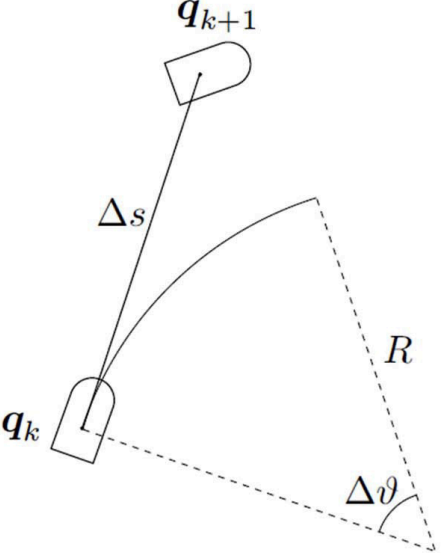
\includegraphics[width=.2\textwidth]{euler}} \quad
\subfloat[RK2法]{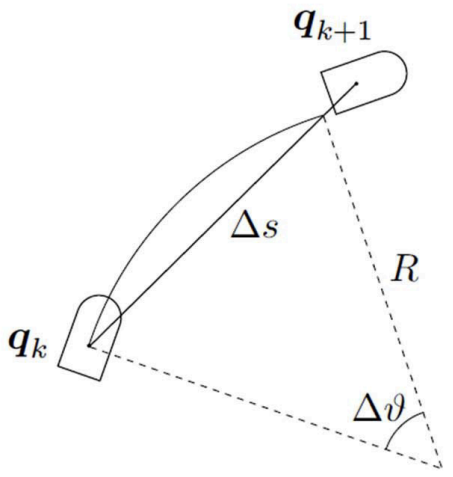
\includegraphics[width=.2\textwidth]{rk2}} \quad
\subfloat[解析积分法]{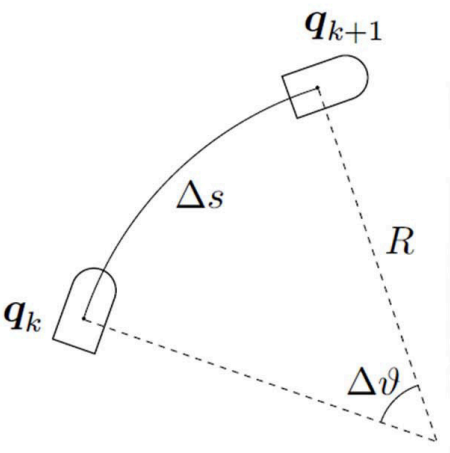
\includegraphics[width=.2\textwidth]{exact}}
\caption{里程计建模方法}
\end{figure}

\begin{itemize}
\begin{minipage}{0.5\textwidth}
\item 欧拉法
$$
\begin{cases}
x_{k + 1} = x_k + v_k T_s \cos \theta_k \\
y_{k + 1} = y_k + v_k T_s \sin \theta_k \\
\theta_{k + 1} = \theta_k + \omega_k T_s
\end{cases}   
$$
\end{minipage}
\begin{minipage}{0.5\textwidth}
\item RK2(二阶Runge-Kutta)法
$$
\begin{cases}
x_{k + 1} = x_k + v_k T_s \cos(\theta_k + \frac{\omega_k T_s}{2}) \\
y_{k + 1} = y_k + v_k T_s \sin(\theta_k + \frac{\omega_k T_s}{2}) \\
\theta_{k + 1} = \theta_k + \omega_k T_s
\end{cases}  
$$
\end{minipage}
\item 解析积分法
$$
\begin{cases}
x_{k + 1} = x_k + \frac{v_k}{\omega_k} (\sin \theta_{k + 1} - \sin \theta_k) \\
y_{k + 1} = y_k - \frac{v_k}{\omega_k} (\cos \theta_{k + 1} - \cos \theta_k) \\
\theta_{k + 1} = \theta_k + \omega_k T_s
\end{cases} 
\overset{\omega_k = 0}{\Longrightarrow}
\begin{cases}
x_{k + 1} = x_k + v_k T_s \\
y_{k + 1} = y_k \\
\end{cases}  
$$
\end{itemize}
%------------------------------------------------
\subsubsection[里程计误差]{里程计误差}
%------------------------------------------------
\paragraph{误差来源}
\begin{itemize}
\item 数值积分误差。
\item 运动学参数误差:速度不恒定,半径误差。
\item 打滑。
\end{itemize}
%------------------------------------------------
\paragraph{误差传播(RK2法)}\tip{误差传播}\label{sec:error back}~\\

位姿更新为:
$$
p' = f(x, y, \theta, \Delta\phi_R, \Delta\phi_L) = 
\begin{bmatrix} x \\ y \\ \theta \end{bmatrix} + 
\begin{bmatrix} \frac{r(\Delta\phi_R + \Delta\phi_L)}{2} \cos(\theta_k + \frac{r[\Delta\phi_R - \Delta\phi_L]}{4d}) \\ \frac{r(\Delta\phi_R + \Delta\phi_L)}{2} \sin(\theta_k + \frac{r[\Delta\phi_R - \Delta\phi_L]}{4d}) \\ \frac{r(\Delta\phi_R - \Delta\phi_L)}{2d} \end{bmatrix}
$$

其中$ \Delta\phi_R,\Delta\phi_L $是控制输入量,有误差协方差矩阵迭代公式:
$$ \sum_{p'} = \underbrace{\nabla_p f \cdot \sum_p \cdot \nabla_p f^T}_{\text{位姿}} + \underbrace{\nabla_{r|l}f \cdot \sum_{\Delta} \cdot \nabla_{r|l}f^T}_{\text{控制输入量}} $$

初始化姿态协方差矩阵$ \sum_{p'} $(可零初始化),其更新量为:
$$
\nabla_p f = \begin{bmatrix}\frac{\partial f}{\partial x} & \frac{\partial f}{\partial y} & \frac{\partial f}{\partial \theta}\end{bmatrix} = 
\begin{bmatrix} 1 & 0 & -\Delta s \sin(\theta_k + \frac{\Delta\theta}{2}) \\ 0 & 1 & \Delta s \cos(\theta_k + \frac{\Delta\theta}{2}) \\ 0 & 0 & 1 \end{bmatrix}
$$

假设$ \Delta\phi_R,\Delta\phi_L $的误差相互独立,有控制输入量协方差矩阵:
$$ \sum_{\Delta} = covar(\Delta\phi_R, \Delta\phi_L) = \begin{bmatrix} k_r||\Delta\phi_R|| & 0 \\ 0 & k_l||\Delta\phi_L|| \end{bmatrix} $$

其更新量为:
$$ \nabla_{rl}f = \begin{bmatrix} \frac{\partial f}{\partial \Delta\phi_R} & \frac{\partial f}{\partial \Delta\phi_L} \end{bmatrix} = \begin{bmatrix} \frac{r}{2}\cos(\theta_k + \frac{\Delta\theta}{2}) - \frac{r}{4d}\Delta s \sin(\theta_k + \frac{\Delta\theta}{2}) & \frac{r}{2}\cos(\theta_k + \frac{\Delta\theta}{2}) + \frac{r}{4d}\Delta s \sin(\theta_k + \frac{\Delta\theta}{2}) \\ \frac{r}{2}\sin(\theta_k + \frac{\Delta\theta}{2}) + \frac{r}{4d}\Delta s \cos(\theta_k + \frac{\Delta\theta}{2}) & \frac{r}{2}\sin(\theta_k + \frac{\Delta\theta}{2}) - \frac{r}{4d}\Delta s \cos(\theta_k + \frac{\Delta\theta}{2}) \\ \frac{r}{2d} & -\frac{r}{2d} \end{bmatrix} $$
%------------------------------------------------
\paragraph{误差转化展示}
原理见\ref{sec:error}。

\begin{figure}[H]
\centering
\subfloat[直线运动]{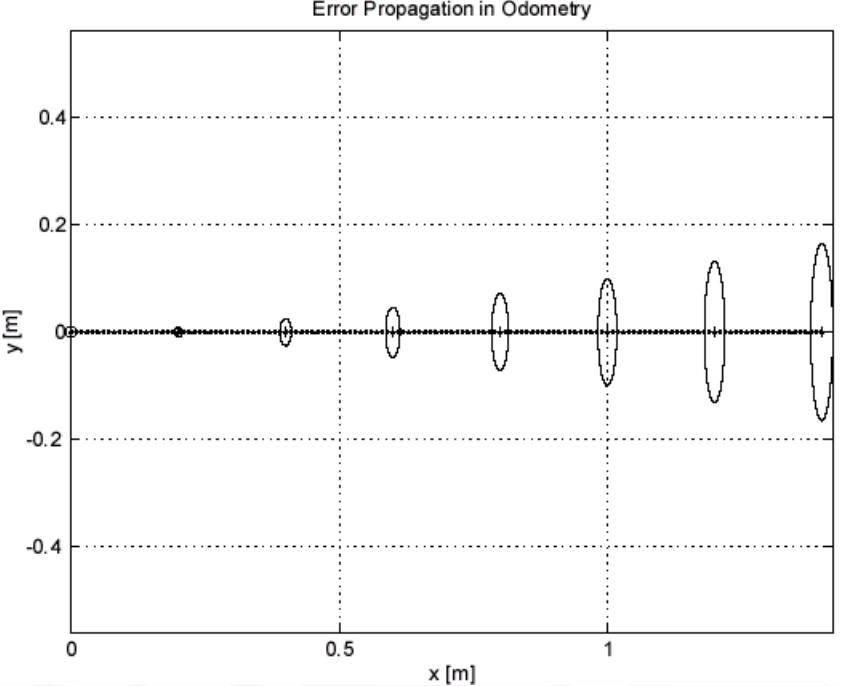
\includegraphics[width=.3\textwidth]{line}} \quad
\subfloat[曲线运动]{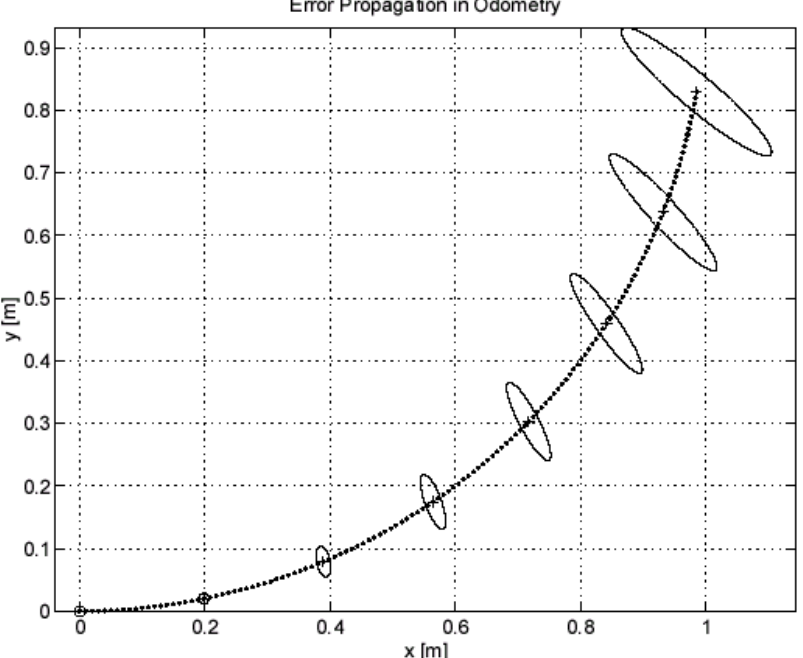
\includegraphics[width=.3\textwidth]{circle}}
\caption{里程计误差转化展示}
\end{figure}

直线运动时误差方向与运动方向垂直,曲线运动时则不垂直。
%------------------------------------------------
\subsection[激光传感器]{激光传感器}
\begin{itemize}
\item 组成:激光器,激光检测器,测量电路。
\item 特点:无接触远距离测量,速度快,精度高,量程大,抗干扰能力强。
\item 激光测距:到达时间法(Time of Flight,TOF):$ \text{时间精度} = \frac{\text{测量精度}}{c(3 \times 10^8)} $。
\item 位移测量:对参考信号和测量信号进行相位测量。
\end{itemize}
%------------------------------------------------
\section{机器人点云处理}
%------------------------------------------------
\subsection[直线提取]{直线提取}
%------------------------------------------------
\subsubsection[最小二乘法]{最小二乘法(Least Squares Method)}
在求解拟合直线时,最小化拟合误差平方和,目标式为:
$$ \min \sum_{i = 1}^{n} d_i^2 = \min \sum_{i = 1}^{n}[y_i - f(x_i)]^2 $$

其中$ f(x) = ax + b $是拟合直线,$ (x, y) $是待拟合的点坐标。
%------------------------------------------------
\paragraph{求解方法}
\begin{enumerate}
\item 求偏导:求目标式关于$ a, b $的偏导,得到如下极值条件:
$$
\begin{cases}
\frac{\partial \Pi}{\partial a} = 2 \sum_{i = 1}^{n} [y_i - (a + bx_i)] = 0 \\
\frac{\partial \Pi}{\partial b} = 2 \sum_{i = 1}^{n} x_i [y_i - (a + bx_i)] = 0 \\
\end{cases}
$$
\item 矩阵形式\tip{最小二乘法矩阵形式求解}:将拟合直线$ f(x) = ax + b $增广为矩阵形式$ Y = X\beta $,在误差$ d = Y - X\beta $趋于$ 0 $时,有$ Y = X\beta $,因此:
$$ Y = X\beta \Rightarrow X^T Y = X^T X\beta \Rightarrow \beta = (X^T X)^{-1}X^T Y $$
\end{enumerate}
%------------------------------------------------
\subsubsection[Split-and-Merge]{Split-and-Merge(分割与合并)\tip{Split-and-Merge直线提取}}
\begin{enumerate}
\item 分裂(Split):以全集作为初始点集。对当前点集拟合直线(采用端点拟合),计算到最远点的距离,距离大于阈值则在该最远点处将点集分裂为两个子集,并对分裂后的两个子集进行迭代。
\item 合并(Merge):检查相邻线段是否满足合并要求(合并后是否有过远点),若满足要求,则合并并拟合新的直线。
\end{enumerate}
%------------------------------------------------
\subsubsection[Line-Regression]{Line-Regression(线性回归)}
\begin{enumerate}
\item 滑动拟合:选取窗口,在其内采用最小二乘法拟合直线,之后滑动窗口拟合新的直线。
\item 合并:检查相邻线段是否满足合并的角度和距离要求,满足则合并并拟合新的直线,直到所有线段不可再合并。
\end{enumerate}
%------------------------------------------------
\subsubsection[RANSAC]{RANSAC(Random Sample Consensus,随机抽样一致性算法)\tip{RANSAC直线提取}}
\begin{itemize}
\item 外点(outliers):异常值。
\item 内点(inliers):符合模型的数据点。
\end{itemize}
\begin{enumerate}
\item 根据内点比例$ w $和找到一个完全由内点组成的样本的希望概率$ p $计算迭代次数:
$$ k = \frac{log(1 - p)}{log(1 - w^2)} $$
\item 从所有数据点中随机选择最小数量(直线2点,平面3点)的数据点子集,确定唯一的模型参数。
\item 计算剩余数据点与该模型的误差,小于设定阈值的为内点。
\item 重复迭代次数次采样,选取包含最多内点的模型。
\end{enumerate}
%------------------------------------------------
\subsubsection[Hough-Transform]{Hough-Transform(霍夫变换)}
图像空间中的一个点对应Hough空间中的一条线。激光定位任务中,常用极坐标$ \rho = x \cos \theta + y \sin \theta $表示。在定距下,误差呈正态分布;而在变距下,误差增长与距离正相关。
\begin{enumerate}
\item 计算数据范围(Hough空间参数分辨率),并初始化累加器。
\item 遍历边缘点,计算可能的参数组合,并在对应位置进行投票。
\item 在累加器中寻找峰值(可能不唯一),获得相应Hough空间参数。
\item 转换回图像空间,确定直线。
\end{enumerate}
%------------------------------------------------
\paragraph{最小二乘直线拟合}~\\

点$ (\rho_i, \theta_i) $到拟合直线$ (r, \alpha) $的距离近似为$ d_i $:
$$ \rho_i \cos(\theta_i - \alpha) - r = d_i $$

使其加权平方和最小,得到最优拟合直线。

误差传播为:
\begin{align*}
C_x = \begin{bmatrix} diag(\sigma_\rho^2) & 0 \\ 0 & diag(\sigma_\theta^2) \end{bmatrix}_{2n \times 2n} &\quad
F_{\rho\theta} = \begin{bmatrix} \frac{\partial \alpha}{\partial \rho_1} & \frac{\partial \alpha}{\partial \rho_2} & \cdots & \frac{\partial \alpha}{\partial \theta_{n - 1}} & \frac{\partial \alpha}{\partial \theta_n} \\ \frac{\partial r}{\partial \rho_1} & \frac{\partial r}{\partial \rho_2} & \cdots & \frac{\partial r}{\partial \theta_{n - 1}} & \frac{\partial r}{\partial \theta_n} \end{bmatrix} \\
C_{\alpha r} &= F_{\rho\theta} C_x F_{\rho\theta}^T    
\end{align*}
%------------------------------------------------
\subsubsection[性能对比]{性能对比}
\begin{table}[H]
\centering
\begin{tabular}{c|ccccc}
\hline
算法 & 复杂度 & 假阳性率FPR & 精度 & 多直线检测 & 属性 \\
\hline
Split-and-Merge & $ n \log n $ & 低 & 低 & 适用 &  \\
Line-Regression & $ n n_f $ & 低 & 低 & 适用 & 有序点云 \\
RANSAC & $ S n k $ & 高 & 高 & 需调整 & 容忍外点 \\
Hough-Transform & $ S n n_C + S n_R n_C $ & 高 & 高 & 适用 &  \\
\hline
\end{tabular}
\caption{直线特征提取算法性能对比}
\end{table}
%------------------------------------------------
\subsection[定位与匹配]{定位与匹配}
%------------------------------------------------
\subsubsection[基于SVD的定位算法]{基于SVD的定位算法\tip{基于SVD的定位算法}}
%------------------------------------------------
\paragraph{条件与目标}~\\

在二维平面上,有基于世界坐标系的点云$ P = \{p_1, p_2, \dots, p_n\} $和基于激光坐标系的点云$ Q = \{q_1, q_2, \dots, q_n\} $,它们按下标顺序匹配,求解刚体变换(旋转阵$ R $和平移量$ t $)。

以误差平方加权和的形式建模,得到目标式:
$$ (R, t) = argmin \sum_{i = 1}^{n}w_i ||(R p_i + t) - q_i||^2 $$

其中$ w_i $表示匹配点对$ (p_i, q_i) $的权重,可取为距离的倒数$ w_i = \frac{1}{\sigma_i(\rho_i)} $。
%------------------------------------------------
\paragraph{加权平均}~\\

为求极值,对目标式求关于$ t $的偏导:
$$ 
2t(\sum_{i = 1}^{n} w_i) + 2R(\sum_{i = 1}^{n} w_i p_i) - 2\sum_{i = 1}^{n} w_i q_i = 0 
\overset{\text{等号两边同除}}{\underset{\sum_{i = 1}^{n} w_i}{\Longrightarrow}}
t + R\frac{(\sum_{i = 1}^{n} w_i p_i)}{\sum_{i = 1}^{n} w_i} - \frac{\sum_{i = 1}^{n} w_i q_i}{\sum_{i = 1}^{n} w_i} = 0
$$

取两个点云的加权中心点$ \hat{p} = \frac{\sum_{i = 1}^{n} w_i p_i}{\sum_{i = 1}^{n} w_i}, \hat{q} = \frac{\sum_{i = 1}^{n} w_i q_i}{\sum_{i = 1}^{n} w_i} $,上式可化简为$ t = \hat{q} - R \hat{p} $。该式描述了平移量和旋转阵的关系,将其带回目标式,得到单变量最值问题:
$$ R = argmin \sum_{i = 1}^{n}w_i ||R(p_i - \hat{p}) - (q_i - \hat{q})||^2 $$
%------------------------------------------------
\paragraph{去中心化}~\\

取去中心化$ x_i = p_i - \hat{p}, y_i = q_i - \hat{q} $,目标式可化简为:
$$ R = argmin \sum_{i = 1}^{n}w_i ||R x_i - y_i||^2 $$

将平方项变成矩阵相乘的形式:
$$ ||Rx_i - y_i||^2 = (R x_i - y_i)^T(R x_i - y_i) = x_i^T (R^T R) x_i - y_i^T R x_i - x_i^T R^T y_i + y_i^T y_i $$
\begin{itemize}
\item 旋转阵为标准正交阵,$ R^{-1} = R^T $,因此$ R^T R = E $。
\item $ x_i^T R^T y_i $是一个$ 1 \times 1 $标量,转置后不变,$ x_i^T R^T y_i = y_i^T R x_i $。
\end{itemize}

所以:
$$ ||Rx_i - y_i||^2 = x_i^T x_i - 2 y_i^T R x_i + y_i^T y_i $$

其中仅有负号项与$ R $相关,其它项都是定值,目标可改写为:
$$ R = argmax \sum_{i = 1}^{n}w_i y_i^T R x_i $$
%------------------------------------------------
\paragraph{SVD分解}\label{sec:svd back}~\\

将其写成对角阵的迹的形式:
\begin{align*}
\sum_{i = 1}^{n} w_i y_i^T R x_i 
&= tr(diag(w_1 y_1^T R x_1, w_2 y_2^T R x_2, \dots, w_n y_n^T R x_n)) \\
&= tr(diag(w_1, w_2, \dots, w_n) \begin{bmatrix} y_1^T & y_2^T & \vdots & y_n^T \end{bmatrix}^T R \begin{bmatrix} x_1 & x_2 & \cdots & x_n \end{bmatrix}) \\
&= tr(WY^TRX)
\end{align*}

因为矩阵的迹满足$ tr(AB) = tr(BA) $,所以$ tr(WY^TRX) = tr(RXWY^T) $。令$ S = XWY^T $,基于SVD原理(见附录\ref{sec:svd}),$ S = U \Sigma V^T $,其中$ U,V $是单位正交阵,$ \Sigma $为对角阵。所以$ tr(RXWY^T) = tr(RU \Sigma V^T) = tr(\Sigma V^TRU) $,后三者都是单位正交阵,它们的积$ M $也是单位正交阵。目标改写为:
$$ R = argmax tr(\Sigma M) $$
%------------------------------------------------
\paragraph{求解$ R $和$ t $}
由于单位正交阵的最大迹是在单位阵下取得的,最大值条件为$ M = E $,即$ R = VU^T $。代回$ R $和$ t $的关系式,可确定$ t $。
%------------------------------------------------
\subsubsection[基于ICP的点云匹配算法]{基于ICP(Iterative Closest Point,迭代最近点)的点云匹配算法\tip{基于ICP的点云匹配算法}}
\begin{enumerate}
\item 条件与目标:求解二维平面上检测点云$ P = \{p_1, p_2, \dots, p_{N_p}\} $和目标点云$ X = \{x_1, x_2, \dots, x_{N_x}\} $的匹配。
\item 计算最近点集:采取采样方法获得目标点云,并采用点集匹配方法为检测点云数据点匹配最近的目标点云数据点。

\begin{minipage}{0.5\textwidth}
\begin{itemize}
\item 均匀采样。
\item 随机采样。
\item 基于特征的采样。
\item 法向量空间采样。
\end{itemize}
\end{minipage}
\begin{minipage}{0.5\textwidth}
\begin{itemize}
\item Closest point Matching(CMP)。
\item Normal Shooting Matching。
\item Point-to-Plane Matching。
\item Projection Matching。
\end{itemize}
\end{minipage}
\item 变换:使用基于SVD的定位算法求解齐次变换矩阵并应用于检测点云。
\item 目标函数计算:统计对齐误差,如果达到阈值则停止迭代,否则重复上述操作。
\end{enumerate}
%------------------------------------------------
\section{机器人定位}
%------------------------------------------------
\subsection[定位与导航]{定位与导航}
%------------------------------------------------
\paragraph{导航}
不能碰障碍物,掌握目标的方向。
\begin{itemize}
\item 基于行为:如沿墙边前进。
\item 基于地图:已知地图,需要定位。
\end{itemize}
%------------------------------------------------
\paragraph{定位}
\begin{itemize}
\item 问题
\begin{itemize}
\item 全局定位:未知初始位置,根据地图进行定位。
\item 位置跟踪:已知初始位置,跟踪位置变化。
\item 绑架问题。
\end{itemize}
\item 方法:基于机载传感器、基于额外传感器和路标、里程计。
\item 分类(不确定度分布):连续单峰(卡尔曼滤波)、连续多峰、离散多峰(粒子滤波)、拓扑。
\end{itemize}
%------------------------------------------------
\subsection[贝叶斯定位]{贝叶斯定位}
%------------------------------------------------
\paragraph{原理}
新信息出现后的概率 = 概率 $ \times $ 新信息带来的调整:
$$ p(x|y) = \frac{p(y|x)p(x)}{p(y)} $$
%------------------------------------------------
\paragraph{思想}
使用低精度传感器(如里程计)跟踪运动状态,不确定度不断提高,定期使用高精度传感器(如激光雷达),修正估计。
%------------------------------------------------
\paragraph{特点}
\begin{itemize}
\begin{minipage}{0.5\textwidth}
\item 连续型
\begin{itemize}
\item 精度受传感器数据限制。
\item 通常是单一假设位姿估计。
\item 对于单一假设发散时会丢失。
\item 表示紧凑,计算资源需求合理。
\end{itemize}
\end{minipage}
\begin{minipage}{0.5\textwidth}
\item 离散型
\begin{itemize}
\item 精度受离散化分辨率限制。
\item 通常是多假设位姿估计。
\item 发散时收敛到另一单元,永不丢失。
\item 需大量内存和计算资源。
\end{itemize}
\end{minipage}
\end{itemize}
%------------------------------------------------
\subsection[基于卡尔曼滤波的定位]{基于卡尔曼滤波的定位}
%------------------------------------------------
\subsubsection[卡尔曼滤波]{卡尔曼滤波}
%------------------------------------------------
\paragraph{推导}
两次独立测量的概率均服从正态分布$ p_1(q) = N(\hat{q}_1, \sigma_1^2), p_2(q) = N(\hat{q}_2, \sigma_2^2) $,它们整合得到的最终分布也服从正态分布:
\begin{align*}
p(q) = p_1(q) \cdot p_2(q) &= \frac{1}{\sigma_1 \sqrt{2\pi}}exp(-\frac{(q - \hat{q}_1)^2}{2\sigma_1^2}) \cdot \frac{1}{\sigma_2 \sqrt{2\pi}}exp(-\frac{(q - \hat{q}_2)^2}{2\sigma_2^2}) \\
&= \frac{1}{2\sigma_1 \sigma_2 \pi}\exp[-\frac{(q - \hat{q}_1)^2}{2\sigma_1^2} - \frac{(q - \hat{q}_2)^2}{2\sigma_2^2}] \\
&= \frac{1}{2\sigma_1 \sigma_2 \pi}\exp\{-\frac{1}{2}[\frac{q^2(\sigma_1^2 + \sigma_2^2) - 2q(\hat{q}_1 \sigma_2^2 + \hat{q}_2 \sigma_1^2) + (\hat{q}_1^2 \sigma_2^2 + \hat{q}_2^2 \sigma_1^2)}{\sigma_1^2 \sigma_2^2}]\} \\
&= \frac{1}{2\sigma_1 \sigma_2 \pi}\exp\{-\frac{1}{2}[\frac{q^2 - \frac{2q(\hat{q}_1 \sigma_2^2 + \hat{q}_2 \sigma_1^2)}{\sigma_1^2 + \sigma_2^2} + \frac{(\hat{q}_1^2 \sigma_2^2 + \hat{q}_2^2 \sigma_1^2)}{\sigma_1^2 + \sigma_2^2}}{\frac{\sigma_1^2 \sigma_2^2}{\sigma_1^2 + \sigma_2^2}}]\} \\
&= \underbrace{\frac{1}{2\sigma_1 \sigma_2 \pi}\exp[-\frac{1}{2}\frac{\frac{\hat{q}_1^2 \sigma_2^2 + \hat{q}_2^2 \sigma_1^2}{\sigma_1^2 + \sigma_2^2} - (\frac{\hat{q}_1 \sigma_2^2 + \hat{q}_2 \sigma_1^2}{\sigma_1^2 + \sigma_2^2})^2}{\frac{\sigma_1^2 \sigma_2^2}{\sigma_1^2 + \sigma_2^2}}]}_{\text{常数}}\underbrace{\exp[-\frac{1}{2}\frac{(q - \frac{\hat{q}_1 \sigma_2^2 + \hat{q}_2 \sigma_1^2}{\sigma_1^2 + \sigma_2^2})^2}{\frac{\sigma_1^2 \sigma_2^2}{\sigma_1^2 + \sigma_2^2}}]}_{\text{正态分布}} \\
&= N(\hat{q}, \sigma^2)
\end{align*}

有:
\begin{align*}
\hat{q} = \underbrace{\frac{\hat{q}_1 \sigma_2^2 + \hat{q}_2 \sigma_1^2}{\sigma_1^2 + \sigma_2^2}}_{\text{方差小的项权重大}} &\Leftrightarrow \hat{q} = \hat{q}_1 + \frac{\sigma_1^2}{\sigma_1^2 + \sigma_2^2}\underbrace{(\hat{q}_2 - \hat{q}_1)}_{\text{校正量}} \\
\sigma^2 = \frac{\sigma_1^2 \sigma_2^2}{\sigma_1^2 + \sigma_2^2} &\Leftrightarrow \sigma^2 = \underbrace{\sigma_1^2 - \frac{\sigma_1^4}{\sigma_1^2 + \sigma_2^2}}_{< \sigma_1^2, \sigma_2^2}
\end{align*}

以$ P = \sigma_1^2, Q = \sigma_2^2, R = \sigma^2 $,记卡尔曼增益$ K = P(P + Q)^{-1} $和创新协方差$ \Sigma_{IN} = P + Q $:
\begin{align*}
\hat{q} &= \hat{q}_1 + P(P + Q)^{-1}(\hat{q}_2 - \hat{q}_1) = \hat{q}_1 + K(\hat{q}_2 - \hat{q}_1) \\
R &= P - P(P + Q)^{-1}P = P - K \cdot \Sigma_{IN} \cdot K^T
\end{align*}

\begin{align*}
&\text{过程(推算)方程:}x_k = A x_{k - 1} + B u_{k - 1} + w_{k - 1} \\
&\text{测量方程:}z_k = H x_k + v_k
\end{align*}

其中$ x_k \in R^n $为系统状态,$ z_k \in R^m $为测量输出,$ u_k \in R^l $为系统输入。$ w_k \in R^n $为过程噪声(Process Noise)$ p(w) = N(0, Q) $,$ v_k \in R^m $为测量噪声(Measurement Noise,白噪声)$ p(v) = N(0, R) $。

有先/后验估计$ \hat{x}_k^-, \hat{x}_k $,先/后验估计误差$ e_k^- = x_k - \hat{x}_k^-, e_k = x_k - \hat{x}_k $,先/后验估计方差$ P_k^- = E[e_k^- e_k^{-T}], P_k = E[e_k e_k^T] $。其中,优化目标是$ argmin_K P_k $。

先后验转化关系为:
$$ \hat{x}_k = \hat{x}_k^- + \underbrace{K}_{\text{卡尔曼增益}}\underbrace{(z_k - H \hat{x}_k^-)}_{\text{新息}} $$

$ P_k $可进行转化:
\begin{align*}
P_k &= E[e_k e_k^T] = E[(x_k - \hat{x}_k)(x_k - \hat{x}_k)^T] (\text{误差展开}) \\
&= E[\{x_k - [\hat{x}_k^- + K(z_k - H\hat{x}_k^-)]\} \{x_k - [\hat{x}_k^- + K(z_k - H\hat{x}_k^-)]\}^T] (\text{代入先后验转化关系}) \\
&= E\{[(x_k - \hat{x}_k^-) - K(H x_k + v_k - H \hat{x}_k^-)][(x_k - \hat{x}_k^-) - K(H x_k + v_k - H \hat{x}_k^-)]^T\} (\text{代入测量方程}) \\
&= E\{[(I - KH)e_k^- - Kv_k][(I - KH)e_k^- - Kv_k]^T\} (\text{误差重构}) \\
&= (I - KH) \underbrace{E[e_k^- e_k^{-T}]}_{P_n^-} (I - KH)^T + K \underbrace{E[v_k v_k^T]}_{R} K^T - K \underbrace{E[v_k e_k^{-T}]}_{\text{不相干,}0} (I - KH)^T -(I - KH) \underbrace{E[e_k^- v_k^T]}_{\text{不相干,}0} K^T \\
&= (I - KH)P_k^-(I - KH)^T + KRK^T
\end{align*}

令偏导为$ 0 $:
$$ \frac{\partial P_k}{\partial K} = -2P_k^- H^T + 2K H P_k^- H^T + 2KR = 0 $$

有$ K = P_k^- H^T(H P_k^- H^T + R)^{-1} $,在方差趋于$ 0 $时,$ \lim_{R \to 0} K = H^{-1}, \lim_{P_k^- \to 0} K = 0 $。
%------------------------------------------------
\paragraph{步骤}\tip{卡尔曼滤波迭代公式}
\begin{figure}[H]
\centering
\begin{tikzpicture}[node distance=3cm, auto, thick]
\usetikzlibrary{positioning}
\node[draw, rectangle, minimum width=5cm, minimum height=2cm, text width=5cm](predict){
\centering 过程
\vspace{-1em}
\begin{align*}
&\hat{x}_k^- = A\hat{x}_{k - 1} + Bu_{k - 1} \\
&P_k^- = AP_{k - 1}A^T + Q
\end{align*}
};
\node[draw, rectangle, minimum width=5cm, minimum height=3cm, text width=5cm, right=of predict] (correct) {
\centering 测量
\vspace{-1em}
\begin{align*}
&K_k = P_k^-H^T(H P_k^- H^T + R)^{-1} \\
&\hat{x}_k = \hat{x}_k^- + K_k(z_k - H \hat{x}_k^-) \\
&P_k = (I - K_k H)P_k^- < P_k^-,R
\end{align*}
};
\node[draw, rectangle, minimum width=5cm, minimum height=2cm, text width=5cm, below=0.5cm of predict] (init) {
\centering 初始化
\vspace{-1em}
\begin{align*}
&\hat{x}_0 = H z_0 \\
&P_0 = \begin{bmatrix} v_{x0} & 0 \\ 0 & v_{y0} \end{bmatrix} 
\end{align*}
};
\draw[->, line width=1pt] (predict) to[bend left=20] (correct);
\draw[->, line width=1pt] (correct) to[bend left=20] (predict);
\draw[->, line width=1pt] (init) to (predict);
\end{tikzpicture}
\caption{卡尔曼滤波框图}
\end{figure}
%------------------------------------------------
\subsubsection[基于卡尔曼滤波的定位算法]{基于卡尔曼滤波的定位算法\tip{基于卡尔曼滤波的定位算法}}
%------------------------------------------------
\paragraph{步骤}
$ Prediction \rightarrow Observation \rightarrow Estimation $

\begin{figure}[H]
\centering 
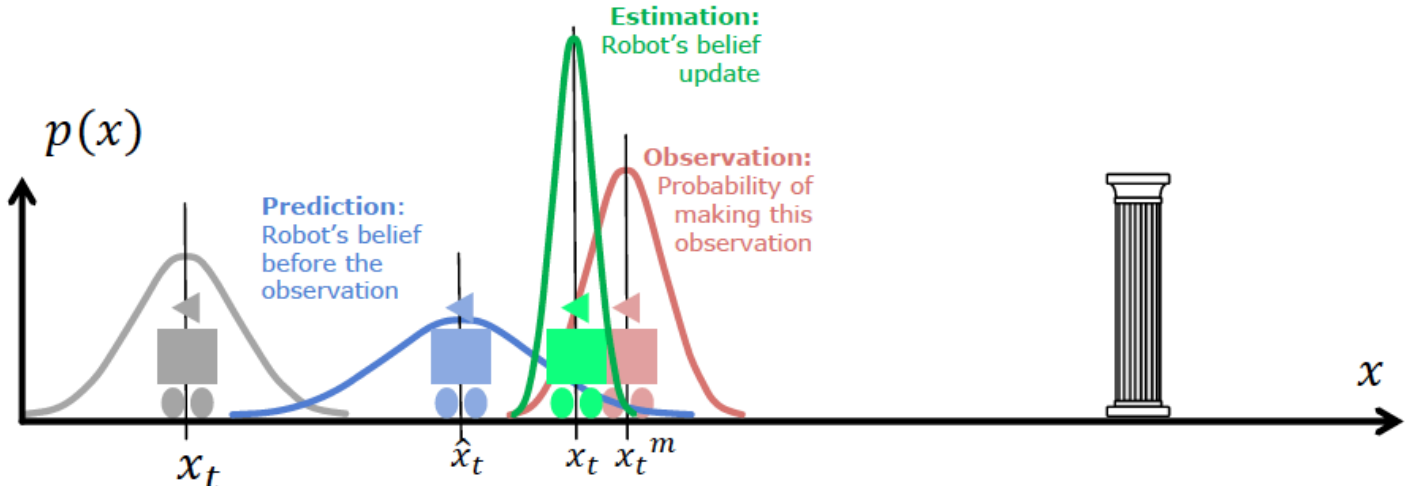
\includegraphics[width=0.8\textwidth]{kalman} 
\caption{基于卡尔曼滤波的定位算法示意图}
\end{figure}

\begin{enumerate}
\item 先验估计:预测模型,如里程计模型。
\item 先验估计误差:误差传导模型。
\item 观测:如激光定位,采用SVD确定位姿,采用ICP配准。
\item 观测误差:SVD匹配误差。
\item 基于观测的后验估计:卡尔曼滤波。
\end{enumerate}
%------------------------------------------------
\paragraph{描述维度}
\begin{table}[H]
\centering
\begin{tabular}{c|c|c|c|c}
\hline
状态 & 状态转移$ A $ & 测量 & 测量矩阵$ H $ & 性能 \\
\hline
$ \begin{bmatrix} x_k \\ y_k \end{bmatrix} $ & $ \begin{bmatrix} 1 & 0 \\ 0 & 1 \end{bmatrix} $ & 
\multirow{2}{*}{$ \begin{bmatrix} u_k \\ v_k \end{bmatrix} $} & $ \begin{bmatrix} u_k \\ v_k \end{bmatrix} $ & 
\begin{tabular}[c]{@{}c@{}}动态误差大\\静止误差小\\适合缓慢移动\end{tabular} \\
\cline{1-2}\cline{4-5}
$ \begin{bmatrix} x \\ y \\ \frac{dx}{dt} \\ \frac{dy}{dt} \end{bmatrix} $ & $ \begin{bmatrix} 1 & 0 & dt & 0 \\ 0 & 1 & 0 & dt \\ 0 & 0 & 1 & 0 \\ 0 & 0 & 0 & 1 \end{bmatrix} $ & 
 & $ \begin{array}{c} \begin{bmatrix} H_x & 0 & 0 & 0 \\ 0 & H_y & 0 & 0 \end{bmatrix} \\ \text{未测量速度} \end{array} $ & 
\begin{tabular}[c]{@{}c@{}}动态误差小\\静止误差大\\低维估计高维\end{tabular} \\
\hline
\end{tabular}
\caption{卡尔曼滤波算法描述维度}
\end{table}
%------------------------------------------------
\paragraph{特点}
\begin{itemize}
\item 严重依赖匹配精度,匹配失败则定位失败,且无法判断和恢复。
\item 收敛速度受初始状态误差和协方差阵精度影响较大。
\item 无法进行全局定位,无法应对绑架问题,只能位置跟踪。
\item 不确定度需为单峰高斯分布。
\end{itemize}
%------------------------------------------------
\subsection[蒙特卡洛定位]{蒙特卡洛定位}
%------------------------------------------------
\subsubsection[蒙特卡洛方法]{蒙特卡洛方法(Monte Carlo Method)}
不断抽样,逐渐逼近的方法。
%------------------------------------------------
\paragraph{特点}
\begin{itemize}
\item 优点:通用。
\item 缺点:收敛速度慢,不精确。
\end{itemize}
%------------------------------------------------
\paragraph{分布函数拟合}
用样本(粒子)分布来处理各种分布。
\begin{itemize}
\item 已知概率分布求粒子分布:采样排除法,概率高的地方采样密集。
\item 未知概率分布求粒子分布:重要性评估,迭代,根据预估分布(以均匀分布开始)洒粒子,再根据结果调整重要性评估(归一化)。
\end{itemize}
%------------------------------------------------
\subsubsection[蒙特卡洛定位算法(粒子滤波算法)]{蒙特卡洛定位算法(粒子滤波算法,MCL)\tip{蒙特卡洛定位算法(粒子滤波算法)}}
多信息融合,提高真值处的重要性。
%------------------------------------------------
\paragraph{重要性采样}~\\

目标分布$ f_i = [p(x_i|z_1, z_2, z_3)] $,根据贝叶斯定理,有:
$$ p(x_i|z_1, z_2, \cdots, z_n) = \frac{\prod_k p(z_k|x_i)p(x_i)}{p(z_1, z_2, \cdots, z_n)} $$

建议分布$ g_i = [p(x|z_i)] $,有:
$$ p(x_i|z_i) = \frac{p(z_i|x_i)p(x_i)}{p(z_i)} $$

有重要性权重:
$$ w_i = \frac{f_i}{g_i} = \frac{p(x_i|z_1, z_2, \cdots, z_n)}{p(x_i|z_i)} = \frac{p(z_i)\prod_{k\neq i}p(z_k|x_i)}{p(z_1, z_2, \cdots, z_n)} $$

令$ \eta = \frac{p(z_i)}{p(z_1, z_2, \cdots, z_n)} $,则有$ w_i \propto \prod_{k\neq i}p(z_k|x_i) $。
%------------------------------------------------
\paragraph{步骤}
在一次迭代($ X_{t - 1} \rightarrow X_t $)中,经历以下过程:
\begin{enumerate}
\item 预测:基于运动模型(建议分布)对粒子进行更新和采样:
$$ x_t^{(i)} = f(x_{t - 1}^{(i)}, u_t) $$
\item 校正:使用传感器模型计算粒子权重:
$$ w_t^{(i)} = p(z_t | x_t^{(i)}) $$
\item 重采样:根据归一化后的权重进行重采样(采用轮盘赌),权重越大的粒子被采样的概率越高。
\end{enumerate}
%------------------------------------------------
\paragraph{激光雷达观测误差模型}
$ m $指地图。
\begin{itemize}
\item 误差
\begin{itemize}
\item 激光雷达测量误差$ p_{hit}(z_t|x_t, m) $。
\item 没有检测到障碍物$ p_{max}(z_t|x_t, m) $:常值分布,返回激光雷达最大测距距离。
$$
p_{max}(z_t|x_t, m) = \begin{cases}
1 & z_t^k = z_{max} \\
0 & otherwise \\
\end{cases}
$$
\item 随机错误$ p_{rand}(z_t|x_t,m) $:均匀分布,返回错误的距离值。
$$
p_{rand}(z_t|x_t, m) = \begin{cases}
\frac{1}{z_{max}} & 0 \leq z_t^k \leq z_{max} \\
0 & otherwise \\
\end{cases}
$$
\item 激光雷达观测误差模型$ p(z_t|x_t, m) $:上述误差的线性组合。
$$ p(z_t|x_t, m) = \alpha_{hit}p_{hit} + \alpha_{max}p_{max} + \alpha_{rand}p_{rand} \quad \alpha_{hit} + \alpha_{max} + \alpha_{rand} = 1 $$
\end{itemize}
\item 物理模型:$ p_{hit}(z_t|x_t, m) $包含随机噪声,一般为高斯分布。
$$
p_{hit}(z_t|x_t, m) = \begin{cases}
N(z_t^{k*}, \sigma_{hit}^2) & 0 \leq z_t^k \leq z_{max} \\
0 & otherwise \\
\end{cases}
$$
\item 可能域(likelihood):$ p_{hit}(z_t|x_t, m) $,将激光束投影到地图中,以距投影最近的点的距离为均值,激光测距偏差为方差。
\begin{itemize}
\item 优点:在线计算量小,平滑性好,收敛性强,更符合实际情况。
\item 缺点:没有明确的物理意义,仅适用于相对静态的环境(如有路标的工厂)。
\end{itemize}
\end{itemize}
%------------------------------------------------
\paragraph{特点}
\begin{itemize}
\item 优点:计算简单,可解决大范围全局定位问题,适用于多种分布。
\item 缺点:粒子数过大时占用内存大,计算效率低;大地图下,只用少量粒子可能发散;无法应对绑架问题。
\end{itemize}
%------------------------------------------------
\subsubsection[自适应蒙特卡洛定位算法]{自适应蒙特卡洛定位算法(AMCL)\tip{自适应蒙特卡洛定位算法}}
%------------------------------------------------
\paragraph{改进}
引入短、长期指数滤波器衰减率$ \alpha_{slow} \ll \alpha_{fast} $,计算短、长期重要性指数似然评价估计$ w_{slow}, w_{fast} $,二者计算公式格式一致,正常时$ w_{slow} < w_{fast} $。
%------------------------------------------------
\paragraph{解决问题}
\begin{itemize}
\item 绑架问题:发生绑架问题时,$ w_{avg} $会突然下降,导致$ w_{slow} > w_{fast} $,将按照概率$ \max(0, 1 - \frac{w_{fast}}{w_{slow}}) $向粒子集中注入随机粒子。
\item 粒子数问题:使用KLD(Kullback-Leibler Divergence,库尔贝克-莱布勒散度,计算概率分布间差异)采样,在趋于收敛的过程中减少粒子。
\end{itemize}
%------------------------------------------------
\paragraph{算法}
其中标红部分是AMCL相较MCL的改进。
\begin{myalgorithm}[AMCL]
\State 参数:$ \alpha_{slow}, \alpha_{fast} $
\State 初始化:初始化$ \overline{X}_t = X_t $为空,初始化$ w_{slow}, w_{fast} $
\For{$ m = 1, \dots, M $}
\State $ x_t^{[m]} = f(u_t, x_{t - 1}^{[m]}) $
\State $ w_t^{[m]} = p(z_t, x_t^{[m]}, \textcolor{red}{m}) $
\State $ \overline{X}_t = \overline{X}_t + \langle x_t^{[m]}, w_t^{[m]} \rangle $
\State \textcolor{red}{$ w_{avg} = w_{avg} + \frac{1}{M} w_t^{[m]} $} \Comment{平均权重}
\EndFor
\State \textcolor{red}{$ w_{slow} = w_{slow} + \alpha_{slow}(w_{avg} - w_{slow}) $} \Comment{慢速权重}
\State \textcolor{red}{$ w_{fast} = w_{fast} + \alpha_{fast}(w_{avg} - w_{fast}) $} \Comment{快速权重}
\For{$ m = 1, \dots, M $}
\State \textcolor{red}{以概率$ \max(0, 1 - \frac{w_{fast}}{w_{slow}}) $向$ X_t $添加随机姿态} \Comment{应对绑架问题}
\State 否则,从$ \overline{X}_t $中按概率$ w_t^{[m]} $采样$ x_t^{[m]} $,并将其添加到$ X_t $ \Comment{重采样}
\EndFor
\State 返回$ X_t $
\end{myalgorithm}
%------------------------------------------------
\section{机器人建图}
%------------------------------------------------
\subsection[地图]{地图}
%------------------------------------------------
\paragraph{功能}
\begin{itemize}
\item 支持机器人进行定位、导航、规划。
\item 容易加入新的信息进行更新。
\item 便于计算机储存和处理。
\end{itemize}
%------------------------------------------------
\paragraph{表示法}
\begin{itemize}
\item 点云地图
\begin{itemize}
\item 优点:可以完全表示环境三维信息,不需要预定义尺寸。
\item 缺点:存储要求高,存在盲区和空洞,需要处理来判断占用和联通状态,不具有通用性(不同机器人无法共用)。
\end{itemize}
\item 栅格地图:以允许误差大小确定栅格大小,用$ 0 - 1 $的值表示栅格被占用的概率(不同激光数据中占用的概率)。
\begin{itemize}
\item 计算
\begin{itemize}
\item 概率:$ p(m_i|s_n) = 1 - E_r E_\alpha $,其中:
$$ E_r = 1 - k_r(\frac{2(\rho_i - r_i)}{\Delta r})^2, E_\alpha = 1 - k_\alpha(\frac{2(\theta_i - \alpha)}{\Delta\alpha})^2 $$
\item 几率:$ \text{几率}l = \frac{\text{概率}p}{1 - \text{概率}p} $,几率与概率非线性正相关。

利用贝叶斯公式得到每次测量(相互独立)的递推关系:
\begin{align*}
p(m_i|s_1, s_2, \cdots, s_n)
& = \frac{p(s_n|m_i, s_1, s_2, \cdots, s_{n - 1})p(m_i|s_1, s_2, \cdots, s_{n - 1})}{p(s_n|s_1, s_2, \cdots, s_{n - 1})} \\
&= \frac{p(s_n|m_i)p(m_i|s_1, s_2, \cdots, s_{n - 1})}{p(s_n)} \\
&= \frac{p(m_i|s_n)p(s_n)p(m_i|s_1, s_2, \cdots, s_{n - 1})}{p(m_i)p(s_n)} \\
&= \frac{p(m_i|s_n)p(m_i|s_1, s_2, \cdots, s_{n - 1})}{p(m_i)}
\end{align*}

有对数几率更新公式:
\begin{align*}
l_{i, n} &= \log\frac{p(m_i|s_1, s_2, \cdots, s_n)}{p(\bar{m}_i|s_1, s_2, \cdots, s_n)} = \log\frac{p(m_i|s_n)p(\bar{m}_i)p(m_i|s_1, s_2, \cdots, s_{n - 1})}{p(\bar{m}_i|s_n)p(m_i)p(\bar{m}_i|s_1, s_2, \cdots, s_{n - 1})} \\
&= \log\frac{p(m_i|s_n)}{p(\bar{m}_i|s_n)} + \underbrace{\log\frac{p(\bar{m}_i)}{p(m_i)}}_{l_0\text{与测量无关}} + \log\frac{p(m_i|s_1, s_2, \cdots, s_{n - 1})}{p(\bar{m}_i|s_1, s_2, \cdots, s_{n - 1})} \\
&= \log\frac{p(m_i|s_n)}{p(\bar{m}_i|s_n)} + \underbrace{l_0}_{\text{占用情况未知时,令}p(m_i) = 0.5, l_0 = 0} + l_{i, n - 1}
\end{align*}
\end{itemize}
\item 特点
\begin{itemize}
\item 优点:可以详细描述环境信息,易于定位和路径规划,不需要预定义尺寸。
\item 缺点:存储要求高,存在盲区和空洞,需要处理来判断占用和联通状态(点占用不够),不具有通用性(不同机器人无法共用)。
\end{itemize}
\item 拓展
\begin{itemize}
\item 2.5维占用栅格地图(扩展高度图):为每个栅格附加高度信息(障碍物最高高度)。
\item 3维占用栅格地图(Voxel Map,体素地图):将空间分解为正方体,判断占用情况。
\item 多分辨率地图:障碍质密处栅格小,无障碍处栅格大,空间占用率高,计算复杂度高,存储存在稀疏特征。
\end{itemize}
\end{itemize}
\item 特征(语义)地图:连续多边形地图,空间占用效率高,定位精度高。
\item 拓扑地图:节点和连线的拓扑结构图,便于导航和路径规划,难以精确定位。
\end{itemize}
%------------------------------------------------
\subsection[SLAM]{SLAM(Simultaneous Localization and Mapping,同步定位与建图)}
%------------------------------------------------
\paragraph{问题描述}
\begin{itemize}
\item 定位(Localization):根据观测序列、运动序列和地图,确定位姿。误差源于全局定位的初始误差和局部定位的观测误差。
$$ E[X^t|Z^t, U^{t - 1}, m] $$
\item 建图(Mapping):根据观测序列和位姿,构建地图。误差源于观测噪声。
$$ E[m|Z^t, X^t] $$
\item SLAM:根据观测序列、运动序列,确定位姿并构建地图。
$$ E[X^t, m|Z^t, U^{t - 1}] $$
\end{itemize}
%------------------------------------------------
\paragraph{SLAM关键}
使用闭环检测进行数据关联,降低估计的不确定度。错误的匹配会使算法发散。
%------------------------------------------------
\paragraph{分类}
\begin{itemize}
\item 基于滤波:EKF-SLAM(卡尔曼滤波)、FastSLAM(粒子滤波,GMAPPING包)。
\item 基于优化:图优化(g2o包),主流。
\end{itemize}
%------------------------------------------------
\subsection[基于滤波的SLAM算法]{基于滤波的SLAM算法}
%------------------------------------------------
\subsubsection[EKF-SLAM]{EKF-SLAM(扩展卡尔曼滤波SLAM)\tip{EKF-SLAM}}
第一个SLAM算法,面向特征地图,采用maximum likelihood进行数据关联。
%------------------------------------------------
\paragraph{状态}
机器人位姿为三维$ X_R = \begin{bmatrix} x & y & \theta \end{bmatrix}^T $,地图特征为二维$ M_i = \begin{bmatrix} x_i & y_i \end{bmatrix}^T $。
\begin{align*}
x_t = \begin{bmatrix} X_R \\ M_1 \\ M_2 \\ \vdots \\ M_n \end{bmatrix}_{(3 + 2n) \times 1} \quad 
\Sigma_t = \begin{bmatrix} 
\Sigma_{X_R} & \Sigma_{X_R m_1} & \Sigma_{X_R m_2} & \cdots & \Sigma_{X_R m_n} \\
\Sigma_{m_1 X_R} & \Sigma_{m_1} & \Sigma_{m_1 m_2} & \cdots & \Sigma_{m_1 m_n} \\
\Sigma_{m_2 X_R} & \Sigma_{m_2 m_1} & \Sigma_{m_2} & \cdots & \Sigma_{m_2 m_n} \\
\vdots & \vdots & \vdots & \ddots & \vdots \\
\Sigma_{m_n X_R} & \Sigma_{m_n m_1} & \Sigma_{m_n m_2} & \cdots & \Sigma_{m_n}
\end{bmatrix}_{(3 + 2n) \times (3 + 2n)}
\end{align*}

高斯协方差矩阵表征了高度互相关性。
%------------------------------------------------
\paragraph{步骤}
\begin{enumerate}
\item 初始状态:$ X_0 = 0, \Sigma_0 = diag(\infty) $。
\item 基于运动模型进行状态估计:地图保持不变,与其相关项为$ 0 $。
\begin{align*}
&\bar{X}_t = f'(X_{t - 1}, U_{t - 1}) \\
&\bar{\Sigma}_{X_R} = \nabla f \cdot \Sigma_{R_{t - 1}} \cdot \nabla f^T + R_t, \quad
\bar{\Sigma}_t = \nabla f' \cdot \Sigma_{R_{t - 1}} \cdot \nabla f'^T + F_x^T R_t F_x, \quad
\nabla f' = \begin{bmatrix} \nabla f & 0 \\ 0 & I \end{bmatrix}
\end{align*}
\item 基于观测模型进行预估观测:每个路标观测独立,交叉项为$ 0 $。
$$
\hat{Z}_t = \begin{bmatrix} Z_{1t} \\ Z_{2t} \\ \vdots \\ Z_{nt} \end{bmatrix}, \quad
Q_t = \begin{bmatrix} Q_{1t} & 0 & \cdots & 0 \\ 0 & Q_{2t} & \cdots & 0 \\ \vdots & \vdots & \ddots & \vdots \\ 0 & 0 & \cdots & Q_{nt} \end{bmatrix}
$$
\item 建立状态估计和预估观测的数据关联。
$$ K_t = \bar{\Sigma}_t H_t^T (H_t \bar{\Sigma}_t H_t^T + Q_t)^{-1} $$
\item 状态更新。
$$ 
X_t = \bar{X}_t + K_t[\hat{Z}_t - h(\bar{X}_t)], \quad
\Sigma_t = [I - K_t H_t]\bar{\Sigma}_t 
$$
\item 获得实际观测:全局地图 = 全局观测位置 + 机器人测量数据。

机器人系的激光观测数据$ z^i_t = [r_t^i, \phi_t^i] $,投影到世界坐标系:
$$ \begin{pmatrix} \bar{x}_m \\ \bar{y}_m \end{pmatrix} = \begin{pmatrix} \bar{x}_R \\ \bar{y}_R \end{pmatrix} + \begin{pmatrix} r_t^i \cos (\phi_t^i + \bar{\theta}_R) \\ r_t^i \sin (\phi_t^i + \bar{\theta}_R) \end{pmatrix} $$

转换得到:
$$
\delta = \begin{pmatrix} \delta_x \\ \delta_y \end{pmatrix} = \begin{pmatrix} \bar{x}_m - \bar{x}_R \\ \bar{y}_m - \bar{y}_R \end{pmatrix}, \quad
q = \delta^T \delta, \quad
\hat{z}_t^i = \begin{pmatrix} \sqrt{q} \\ atan2(\delta_y, \delta_x) - \bar{\theta}_R \end{pmatrix}
$$

有单路标雅可比:
\begin{align*}
H_i^j &= ^{low}H_i^j F_{x, j} \\
&= \frac{1}{q} \begin{pmatrix} -\sqrt{q}\delta_x & -\sqrt{q}\delta_y & 0 & \sqrt{q}\delta_x & \sqrt{q}\delta_y \\ \delta_y & -\delta_x & -q & -\delta_y & \delta_x \end{pmatrix} 
\begin{pmatrix} 
I_3 & 0_{2j - 2} & 0 & 0_{2N - 2j}  \\
0 & 0 & I_2 & 0 \\
\end{pmatrix}
\end{align*}
\item 在地图中加入新的路标:新路标与原路标不独立,因为前者由不确定度决定,而不确定度有后者计算。
\begin{align*}
&m_{n + 1} = f(X_R, Z_{n + 1}) \\
&\nabla f_R = \frac{\partial f(X_R, Z_{n + 1})}{\partial X_R}, \quad \nabla f_Z = \frac{\partial f(X_R, Z_{n + 1})}{\partial Z_{n + 1}} \\
&\Sigma_{m_{n + 1}} = \nabla f_R \cdot \Sigma_{X_R} \cdot \nabla f_R^T + \nabla f_Z \cdot Q_{Z_{n + 1}} \cdot \nabla f_Z^T \\\
&\Sigma_{m_{n + 1}m_i} = \nabla f_R \cdot \Sigma_{X_R m_i} \\
&\Sigma_{m_{n + 1}X_R} = \nabla f_R \cdot \Sigma_{X_R}
\end{align*}

得到新的状态(标红部分为扩充内容):
\begin{align*}
X_t = \begin{bmatrix} X_R \\ M_1 \\ M_2 \\ \vdots \\ M_n \\ \color{red} M_{n + 1} \end{bmatrix}, \quad
\Sigma_t = \begin{bmatrix} 
\Sigma_{X_R} & \Sigma_{X_R m_1} & \cdots & \Sigma_{X_R m_n} & \color{red}\Sigma_{X_R m_{n + 1}} \\
\Sigma_{m_1 X_R} & \Sigma_{m_1} & \cdots & \Sigma_{m_1 m_n} & \color{red}\Sigma_{m_1 m_{n + 1}} \\
\Sigma_{m_2 X_R} & \Sigma_{m_2 m_1} & \cdots & \Sigma_{m_2 m_n} & \color{red}\Sigma_{m_2 m_{n + 1}} \\
\vdots & \vdots & \ddots & \vdots & \color{red}\vdots \\
\Sigma_{m_n X_R} & \Sigma_{m_n m_1} & \cdots & \Sigma_{m_n} & \color{red}\Sigma_{m_n m_{n + 1}} \\
\color{red}\Sigma_{m_{n + 1} X_R} & \color{red}\Sigma_{m_{n + 1} m_1} & \color{red}\cdots & \color{red}\Sigma_{m_{n + 1} m_n} & \color{red}\Sigma_{m_{n + 1}}
\end{bmatrix}
\end{align*}
\item 重复2-7步。
\end{enumerate}
%------------------------------------------------
\paragraph{特点}
\begin{itemize}
\item 计算复杂度高。
\item 要求高斯分布,只能处理单峰假设。
\item 依赖数据关联正确性。
\item 仅适用于有全连接人工路标的点云地图或特征地图,无法使用栅格地图。
\end{itemize}
%------------------------------------------------
\subsubsection[FastSLAM]{FastSLAM(粒子滤波SLAM)\tip{FastSLAM}}
集成粒子滤波器与EKF,使用粒子分布表示位姿。
%------------------------------------------------
\paragraph{粒子降维}
每个粒子相当于对机器人路径的一个假设,构建独立的地图,协方差矩阵只有对角线。
$$ x = (\underbrace{x_1, \cdots, x_t}_{3t\text{,撒粒子获得}}, \underbrace{l_{1, x}, l_{1, y}, \cdots, l_{N, x}, l_{N, y}}_{2N\text{,计算获得}})^T $$

基于饶布莱克维尔定理进行因式分解:
\begin{align*}
p(x_{0:t}, \underbrace{l_{1:M}}_{\text{地图(路标)}}|z_{1:t}, u_{1:t}) 
&= \underbrace{p(x_{0:t}|z_{1:t}, u_{1:t})}_{\text{根据观测定位}} \underbrace{p(l_{1:M}|x_{0:t}, z_{1:t}, u_{1:t})}_{\text{根据观测建图}} \\
&= \underbrace{p(x_{0:t}|z_{1:t}, u_{1:t})}_{\text{粒子滤波}} \underbrace{\Pi_{i = 1}^M p(l_i|x_{0:t}, z_{1:t}, u_{1:t})}_{\text{M个独立2维EKF}}
\end{align*}

其中粒子滤波部分不需要修正过去位姿信息,只需要维护当前位姿。
%------------------------------------------------
\paragraph{步骤}
\begin{enumerate}
\item 运动更新。
\item 计算新特征的EKF。
\item 地图更新。
\item 基于观测计算权重:仅与当前观测相关。
\begin{align*}
w^{[k]} &= \frac{\overbrace{p(x_{1:t}^{[k]}|z_{1:t}, u_{1:t})}^{\text{目标分布}}}{\underbrace{p(x_{1:t}^{[k]}|z_{1:t - 1}, u_{1:t})}_{\text{建议分布}}} \\
&= \frac{\eta p(z_t | x_{1:t}^{[k]}, z_{1:t - 1})p(x_t^{[k]}|x_{t - 1}, u_t)p(x_{1:t - 1}^{[k]}|z_{1:t - 1}, u_{1:t - 1})}{p(x_t^{[k]}|x_{t - 1}, u_t)p(x_{1:t - 1}^{[k]}|z_{1:t - 1}, u_{1:t - 1})} \\
&= \eta p(z_t|x_{1:t}^{[k]}, z_{1:t - 1})
\end{align*}
\item 插入新特征。
\item 基于权重重采样。
\end{enumerate}
%------------------------------------------------
\paragraph{数据关联}
计算观测特征和地图特征的匹配概率,准的粒子概率高,不会因关联错误而全盘错误。
\begin{itemize}
\item 选择概率大的进行匹配。
\item 按照概率进行随机匹配。
\end{itemize}
%------------------------------------------------
\paragraph{特点}
\begin{itemize}
\item 降维高效。
\item 随机采样使数据关联更鲁棒,利用多假设分析忽略位姿误差。
\item 粒子数量选取:尽量多,过多可能占用过大内存,过少可能导致错误。
\end{itemize}
%------------------------------------------------
\subsection[基于优化的SLAM算法]{基于优化的SLAM算法}
图优化SLAM:位姿通过约束相互连接,表征不确定性,寻求最优的节点构型使约束误差最小。
%------------------------------------------------
\paragraph{构建图(前端)}
\begin{itemize}
\item 节点(Node):机器人位姿,包含位姿$ x_{1:n}(x, y ,\theta) $、特征或路标$ m_{1:k}(x, y) $信息。
\begin{itemize}
\item 定位(Pose):$ x^T = (x_1^T, x_2^T, \cdots, x_n^T) \in R^{3n} $。
\item SLAM(Pose feature):$ x^T = (x_1^T, x_2^T, \cdots, x_n^T, m_1^T, m_2^T, \cdots, m_K^T) \in R^{3n + 2K} $。
\end{itemize}
\item 边(Edge):位姿间的空间约束,齐次坐标。
\begin{itemize}
\item 里程计测量$ (X_i^{-1}X_{i + 1}) $和观测$ (X_i^{-1}X_j) $。
\item 信息矩阵:节点间空间约束的不确定性,优化的权重。协方差的逆,值越大相关性越高,越应重视。
\end{itemize}
\end{itemize}
%------------------------------------------------
\paragraph{图优化(后端)}
\begin{itemize}
\item 定位:$ e_{ij}(x_i, x_j) = t2v[z_{ij}^{-1}(x_i^{-1}x_j)] \overset{e_{ij}(x_i, x_j) = 0}{\Longrightarrow} z_{ij} = (x_i^{-1}x_{i + 1}) $。
\item SLAM:$ e_{ij}(z_i, x_j) = \hat{z}_{ij} - z_{ij} = R_j^T(z_i - t_j) - z_{ij} \overset{e_{ij}(x_i, x_j) = 0}{\Longrightarrow} z_{ij} = R_i^T(z_i - t_j) $。
\end{itemize}
%------------------------------------------------
\paragraph{例题}\tip{图优化例题}
\begin{figure}[H]
\centering
\subfloat[定位]{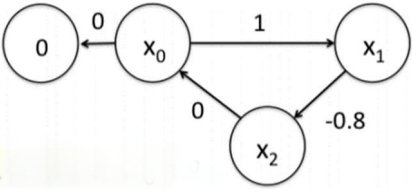
\includegraphics[width=.3\textwidth]{Pose}} \quad
\subfloat[SLAM]{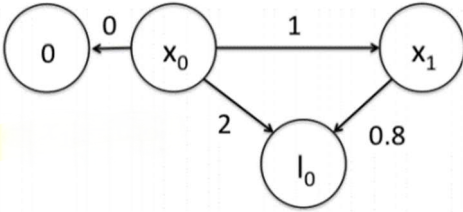
\includegraphics[width=.3\textwidth]{Pose feature}}
\caption{图优化例题}
\end{figure}

\begin{enumerate}
\item 定位:起点在0处,向前移动到达远点,编码器测得位移1m,向后移动回到起点(闭环检测),编码器测得位移0.8米。

有目标函数:
$$ c = \sum_{i = 1}^{4} f_i^2 = (x_0 - 0)^2 + (x_1 - x_0 - 1)^2 + [x_2 - x_1 -(-0.8)]^2 +(x_2 - x_0 - 0)^2 $$

求偏导的得到方程组,解得:
$$
\begin{bmatrix}  x_0 \\ x_1 \\ x_2 \end{bmatrix} 
= \begin{bmatrix} 3 & -1 & -1 \\ -1 & 2 & -1 \\ -1 & -1 & 2 \end{bmatrix}^{-1}
\begin{bmatrix} -1.0 \\ 1.8 \\ -0.8 \end{bmatrix} 
= \begin{bmatrix} 0 \\ 0.93 \\ 0.07 \end{bmatrix}
$$
\item SLAM:起点在0处,观测到前方2m处有路标。向前移动到路标前0.8m处,编码器测得位移1m。

有目标函数:
$$ c = \sum_{i = 1}^{4} f_i^2 = (x_0 - 0)^2 + (x_1 - x_0 - 1)^2 + (l_0 - x_0 - 2)^2 +(l_0 - x_1 - 0.8)^2 $$

求偏导的得到方程组,解得:
$$
\begin{bmatrix}  x_0 \\ x_1 \\ l_0 \end{bmatrix} 
= \begin{bmatrix} 3 & -1 & -1 \\ -1 & 2 & -1 \\ -1 & -1 & 2 \end{bmatrix}^{-1}
\begin{bmatrix} -3.0 \\ 0.2 \\ 2.8 \end{bmatrix} 
= \begin{bmatrix} 0 \\ 1.07 \\ 1.93 \end{bmatrix}
$$
\end{enumerate}
%------------------------------------------------
\paragraph{优化求解}
略
%------------------------------------------------
\paragraph{特点}
\begin{itemize}
\item 仅将实际发生关联的约束构建连接并进行优化,且不是每次观测都需要更新(多分辨率),效率高。
\item 优化思想而非概率思想,易理解和计算。
\end{itemize}
%------------------------------------------------
\subsection[LOAM]{LOAM}
基于激光和里程计。
\begin{itemize}
\item 运动畸变矫正:点云时间戳对齐,利用IMU信息(无IMU时假设匀速)。
\item 特征点提取:平面点、边缘点。
\item 双odom:高频低精度和低频高精度结合。
\end{itemize}
%----------------------------------------------------------------------------------------
\section{机器人运动规划}
%------------------------------------------------
\subsection[运动规划]{运动规划(Motion Planning)}
%------------------------------------------------
\paragraph{需求}
\begin{itemize}
\item 安全性:规避障碍物。
\item 可达性:从起点到终点的连通域。
\item 光滑性:平稳舒适地运行。
\item 可执行性:动力学约束和执行单元的性能约束。
\end{itemize}
%------------------------------------------------
\paragraph{分层规划}
\begin{itemize}
\item 路径规划:只考虑几何约束,不考虑机器人和执行器约束。
\begin{itemize}
\item 基于图搜索:算法完备,有限时间内返回解或返回无解。
\item 基于采样:概率完备。
\end{itemize}
\item 轨迹规划:在给定路径上考虑机器人和执行器约束,生成随时间变化的运动序列。
\begin{itemize}
\item 在线。
\item 离线
\end{itemize}
\end{itemize}
%------------------------------------------------
\subsection[基于图搜索的路径规划]{基于图搜索的路径规划}
%------------------------------------------------
\subsubsection[静态路径规划]{静态路径规划}
%------------------------------------------------
\paragraph{图的构建}
\begin{itemize}
\item 可视图(visibilty graph):连线障碍物顶点和起点终点,找最短路径。可实现无碰撞最短路径距离规划,但太靠近障碍物。
\item 维诺图(Voronoi graph):路径距周围两个最近障碍物等距(L1/L2)。最大化与障碍物的距离,安全但较长。
\item Bug算法图:起点和重点连线,在障碍物处沿边缘行走,更新起点迭代。
\item 精确单元分解地图。
\item 栅格地图:关联格间无障碍。
\item 拓扑地图。
\item 搜索树。
\end{itemize}
%------------------------------------------------
\paragraph{算法}\tip{图搜索算法}
\begin{table}[H]
\centering
\begin{tabular}{|p{2cm}|p{6cm}|p{1.4cm}|p{3.5cm}|p{2cm}|}
\hline
算法 & 原理 & 完备性 & 最优性 & 补充 \\
\hline
深度优先(DFS) & 分支遍历 & 完备 & 不最优 & 无方向性,效率低下 \\
\hline
宽/广度优先(BFS,泛洪搜索) & 层次遍历 & 完备 & 不最优 & 无方向性,效率低下 \\
\hline
Dijkstra & 计算节点到起点的代价,优先遍历队列中代价最小的节点 & 完备 & 最优 & 地图信息利用不充分 \\
\hline
A* & 路径评价由移动开销$ G(n) $和启发函数代价估计$ H(n) $组合得到 & 完备 & 最优(需满足可采纳性和一致性) & 高效,多解,不一定平滑 \\
\hline
\end{tabular}
\caption{图搜索算法对比}
\end{table}

启发函数:
\begin{itemize}
\item 可选:曼哈顿距离、欧几里得距离、切比雪夫距离。
\item 可采纳性:低估代价。
\item 一致性:符合三角不等式。
\item 选取优劣是算法效率的重要因素。
\end{itemize}
%------------------------------------------------
\paragraph{算法补充}
\begin{itemize}
\item 权重A*:为启发函数添加权重$ \epsilon \geq 1 $,限制扩展节点,提高效率,但不满足可采纳性,只能得到局部最优。
\item ARA*(任意时间法+权重A*):快速得到次优,再优化。
\end{itemize}
%------------------------------------------------
\subsubsection[动态路径规划]{动态路径规划}
%------------------------------------------------
\paragraph{动态环境特点}
\begin{itemize}
\item 运行过程中地图可能改变,有动态障碍物。
\item 一般性环境,更符合实际。
\item 需降低复杂度,提高实时性。
\end{itemize}
%------------------------------------------------
\paragraph{算法}
\begin{itemize}
\item D*(动态A*):由目标点向当前位置Dijkstra,利用变化前的地图信息进行动态规划。
\item Fucussed D*:将D*的Dijkstra改为A*。
\item LPA*:增量式搜索。
\item D*-Lite:LPA*的动态形式。
\item AD*:结合ARA*和D*-Lite。
\end{itemize}
%------------------------------------------------
\subsection[基于采样的路径规划]{基于采样的路径规划}
%------------------------------------------------
\paragraph{概述}
\begin{itemize}
\item 采样:在障碍物处密集采样。
\item 距离评估。
\item 碰撞检测:凸障碍已比较完善,非凸障碍尚未完善。
\end{itemize}
%------------------------------------------------
\paragraph{PRM(概率路图)}
略
%------------------------------------------------
\paragraph{RRT(快速探索随机树)}
\begin{itemize}
\item RRT:迭代撒点,选择离目标近的点,按照这个方向步进(不一定到达),更新起点;最后到达终点附近,无法准确到达重点。完备而高效,但是只能得到可行解而非最优解。
\item RRT*:在路径的大圈中进行局部优化,重构节点关系,使局部最优。
\item Informed RRT*:在起点终点连线为主轴的椭圆中进行优化。
\end{itemize}
%------------------------------------------------
\subsection[面向碰撞的局部路径规划]{面向碰撞的局部路径规划}
\begin{itemize}
\item DWA(Dynamic Window Approach):评价函数对方向角、空隙、速度进行加权。计算复杂度低,但可能得不到全局最优。
\item TEB(Timed Elastic Band):连接起点终点为可变形路径,将约束视作引起形变的外力。
\end{itemize}
%------------------------------------------------
\subsection[路径平滑]{路径平滑}
\begin{itemize}
\item 约束:初始、终止状态约束。曲线光滑。
\item 曲线形态:圆弧、贝塞尔曲线。
\end{itemize}
%------------------------------------------------
\subsection[轨迹规划]{轨迹规划}
\begin{itemize}
\item 目标:在执行器约束下,沿给定光滑曲线的可执行的运动命令序列。
\item 约束:初始、终止状态约束,执行器约束,运动学约束。
\end{itemize}
%----------------------------------------------------------------------------------------
\section{附录}
%------------------------------------------------
\subsection[误差转化展示]{误差转化展示}\label{sec:error}
将误差传播协方差矩阵$ \sum_p $转化成椭圆展示。
%------------------------------------------------
\paragraph{计算}
取$ \sum_p $左上二阶子阵$ \sum_{p_{xy}} = \begin{bmatrix} \sigma_{xx} & \sigma_{xy} \\ \sigma_{xy} & \sigma_{yy} \end{bmatrix} $,计算特征值$ \lambda_1,\lambda_2 $和特征向量$ \overrightarrow{p}_1,\overrightarrow{p}_2 $,其分别表示长短轴的大小和方向,圆心是$ (x_k, y_k) $(直接对$ \sum_p $求取特征根和特征向量,再取前两个,结果与其不同)。
%------------------------------------------------
\paragraph{意义}
\begin{itemize}
\item 长短轴表示误差在不同方向上的大小,可通过开根号、乘系数等方法调节。
\item 方向角表示误差传播的主要方向,体现了误差传播的各向异性。
\item 椭圆大小反映了系统的误差范围,可按置信度缩放。
\end{itemize}

返回里程计\ref{sec:error back}。
%------------------------------------------------
\subsection[奇异值分解]{奇异值分解(Singular Value Decomposition,SVD)}\label{sec:svd}
根据$ A_{m \times n} $计算$ (A^T A)_{n \times n} $ 和$ (AA^T)_{m \times m} $两个对称矩阵,求二者的特征值和特征向量:
$$ A^T A v_i = \lambda_i v_i, i = 1, 2, \dots, n \quad AA^T u_i = \mu_i u_i, i = 1, 2, \dots, m $$

其中,$ \lambda_i, \mu_i $是特征值,$ v_i, u_i $是其对应的特征向量,分别组成$ V = [v_1, v_2, \dots, v_n] $和$ U = [u_1, u_2, \dots, u_m] $。

奇异值$ \sigma_i $是$ \lambda_i, \mu_i $的平方根,将其按降序排列,并构造对角矩阵$ \Sigma = diag(\sigma_1, \sigma_2, \dots, \sigma_r) $,得到SVD分解$ A = U \Sigma V^T $。

返回里程计\ref{sec:svd back}。
%----------------------------------------------------------------------------------------
\end{document}